\chapter{Constant-Modulus Algorithm via Wirtinger Flow}
\label{chap:WF}

In this chapter, we introduce the non-convex iterative optimization approach known as Wirtinger Flow, originally proposed for a seemingly different problem known as Phase Retrieval. First, we describe the phase retrieval, to then draw connections between Phase Retrieval and CMA blind estimation, and apply known results from the former into the latter. The most interesting results are related to the \textit{local} convergence properties of CMA, which in turn can help define a more aggresive stepsizes in gradient-descent schemes, ultimately helping in the convergence speed of CMA.


\section{Phase Retrieval}
A recent stream of nonconvex optimization procedures have been developed in the last years for solving quadratic equations, in particular for the phase retrieval problem. The phase retrieval problem can be stated as the recovery of an unknown signal $\bm{z}$ using known sampling vectors $\bm{a}_k$ by the magnitude measurements of the sampled signal only, i.e., $y_k=|a_k\herm z|^2$. The recovery is done by the means of minimizing the error, which is modeled with a smooth cost function to solve the following optimization problem:
\begin{equation}
\min_{\bm{z}\in\mathbb{C}^M}\quad p(\bm{z})=\frac{1}{K}\sum_{k=1}^K\big(|\bm{a}_k\herm\bm{z}|^2-y_k\big)^2. \label{eqn:phaseretrieval}
\end{equation}

Note that in a mathematical sense, phase retrieval is equivalent to the CMA problem in Eq.(\ref{eqn:cma}), by setting $y_r=R_2$ and $\bm{a_k}=\bm{x}_k$, $k\in\{1,\ldots,K\}$, and having $\bm{z}$ as the unknown variable. This similarity inspires the study of the literature on phase retrieval and derive connections between optimization methods for phase retrieval and the CMA problem. However, there are some fundamental differences. First, in phase retrieval there is knowledge of the sampled signal $y_k$, which is closely related to the ground truth and is used thoroughly in the convergence analysis, whereas in CMA-based blind beamforming we have no information of the ideal combiner solution. Second, in phase retrieval there is only one solution (up to scalar rotations), where in blind beamforming, there are as many ideal combiners as transmitter sources (up to scalar rotations), which presents new problems as well. %We will address this drawbacks in our analysis.

\subsection{Wirtinger Flow in Phase Retrieval}
For such a problem formulation, the \textit{Wirtinger Flow} algorithm (WF) presented in \cite{Candes2015a_phaseretrievalWF} has received considerable attention as it guarantees convergence to a solution via gradient-descent with only $\mathcal{O}(M\log M)$ measurements with Gaussian sampling vectors, obtaining  $\epsilon$-accuracy within $\mathcal{O}(KM^2\log\epsilon)$ iterations. This algorithm has received significant research attention and several works have improved WF for the phase retrieval problem \cite{Chen2015truncatedwf,Zhang2017reshapedwf,Bostan2018AcceleratedWF} or adapted WF for different problems \cite{Dong2018blinddemixingwf,Dong2018otacompwf}. 

In more detail, WF is a two stage approach consisting in spectral initialization and gradient descent updates. The former is a method that provides (with high probability) an initial candidate that is located in the most-likely basin of attraction, where a strong minima should be located; whereas the latter is characterized by the notion of Wirtinger calculus (also known as $\mathbb{CR}$-calculus \cite{Kreutz2009wirtinger}), where the strict concept of complex differentiability is dismissed to generalize the derivatives of functions with complex variables, which can then be treated as functions of both the complex variables and their conjugates as independent variables. In particular, this approach provide expressions for the derivatives that closely resemble the results one expects with real variables, thus facilitating the process of obtaining the expressions for gradients and Hessians. Moreover, in the case of any real-valued function $p$ of complex variable $z$, its derivatives satisfy
\begin{equation}
\overline{\bigg({\frac{\partial p}{\partial z}}\bigg)}=\frac{\partial \overline{p}}{\partial \overline{z}}=\frac{\partial p}{\partial \overline{z}}
\end{equation}
and there is no need to compute the derivatives with respect to $\overline{z}$, as the do not provide additional information \cite{Kreutz2009wirtinger}. 

The Wirtinger Flow for phase retrieval, as stated in \cite{Candes2015a_phaseretrievalWF}, is summarized in Algorithm~\ref{alg:wf_pr}.
\begin{algorithm}[H]
	\caption{Wirtinger Flow for Phase Retrieval}
	\label{alg:wf_pr}
	\begin{algorithmic}[1]
		\Statex {\textbf{Given: } Sampling vectors $\bm{a}_k,\,k=1,\ldots,K$, number of iterations $T$ and stepsize $\mu$}
		\Statex \textbf{A) Spectral Initialization:}
		\State{Compute $\displaystyle \eta=\sqrt{\frac{M\sum_k y_k}{\sum_k\|\bm{a}_k\|_2^2}}$}
		\State{Let $\hat{\bm{v}}_1$ be the normalized eigenvector corresponding to the largest eigenvalue of $\bm{Y}=\frac{1}{K}\sum_{k=1}^Ky_k\bm{a}_k\bm{a}_k\herm$}
		\State Set $\bm{z}_0=\eta\hat{\bm{v}}_1$ 
		\Statex \textbf{B) Gradient Descent:}
		\For{$t=0,\ldots,T-1$}
		\State $\displaystyle \bm{z}_{t+1}=\bm{z}_t-\frac{\mu}{\|\bm{z}_t\|_2^2}\nabla p(\bm{z}_t)$
		\EndFor
	\end{algorithmic}
\end{algorithm}

\subsection{Wirtinger Flow for Blind Beamforming}
Using $\mathbb{CR}$-calculus, the gradient of the CMA objective function $f$ can be defined as
\begin{equation}
\nabla_{\bm{w}}f(\bm{w})=\frac{4}{K}\sum_{k=1}^K\Big(|\bm{x}_k\herm\bm{w}|^2-R_2\Big)\bm{x}_k\bm{x}_k\herm\bm{w} \label{eqn:wfgradient}
\end{equation}
and the gradient descent rule with Wirtinger Flow (dismissing the factor 4) is 
\begin{equation}
\bm{w}_{t+1}=\bm{w}_t-\frac{\mu}{K\|\bm{w}_t\|_2^2}\sum_{k=1}^K\Big(|\bm{x}_k\herm\bm{w}|^2-R_2\Big)\bm{x}_k\bm{x}_k\herm\bm{w}_t, \label{eqn:wfupdaterule}
\end{equation}
where the stepsize $\mu$ can be constant or vary, either as a predefined function of the iteration $t$ \cite{Candes2015a_phaseretrievalWF} or using an iterative approach such as line-search, among other methods.

This gradient rule, which notably has a normalization by the norm of the iterate, has in fact been introduced for the CMA problem before in a scheme known as Normalized CMA \cite{Jones1995ncma,Tanrikulu1997ncma,Dogancay2001ncmapartialupdates}. The idea, which comes from normalized LMS algorithm, is to adjust the stepsize in such a way that the updated filter coefficients produce zero error with the current data vector. Nevertheless, these works have not thoroughly studied how to select the stepsize, still relying in trial-and-error to define a stepsize. With the introduction of WF, we aim to prove that we can select the stepsize according to the local geometry of CMA, and therefore improving the speed of the algorithm.

Respect to the spectral initialization proposed by WF for phase retrieval \cite{Candes2015a_phaseretrievalWF}, the eigendecomposition of the sample covariance matrix is highly correlated with the ground truth of the problem (in expectation), and the theory of WF proves that this initialization yields an initial iterate close to the ground truth with high probability. However, if we try to directly apply this initialization scheme in the CMA formulation, the solutions are not readily obtainable from the eigendecomposition. To show this, we derive the sample covariance matrix in the same fashion as WF for phase retrieval, where the known observations are given by the inputs $\bm{x}_k$ and the desired outcomes are equal to the magnitude of the desired modulus of the output signal $R_2$, thus
\begin{equation}
\bm{O}=\frac{1}{K}\sum_{k=1}^KR_2\bm{x}_k\bm{x}_k\herm=\frac{R_2}{K}\sum_{k=1}^K\bm{x}_k\bm{x}_k\herm.
\end{equation}
Consider now the noiseless case, and assume that all transmitted signals have the same transmission power $E_s$ for simplicity.  Taking expectation,
\begin{equation}
\mathbb{E}\{\bm{O}\}=\frac{R_2}{K}\sum_{k=1}^K\bm{H}\mathbb{E}\{\bm{s}_k\bm{s}_k\herm\}\bm{H}\herm=R_2E_s\bm{H}\bm{H}\herm,
\end{equation}
result that depends on the channel but is not explicitly dependent on the solutions. By means of Eq.(\ref{eqn:combineroutput}), these solutions are of the form
\begin{equation}
	\hat{\bm{w}}\herm\bm{x}_k=\hat{\bm{w}}\herm\bm{H}\bm{s_k}=\bm{e}_{l}\herm\bm{s}_k=s_l(k),\quad\text{for some } l\in\{1,\ldots,L\}
\end{equation}
and thus the optimal combiners 
%correspond to the columns of the conjugate transpose of the pseudoinverse of $\bm{H}$, that is,
%\begin{equation}
%\hat{\bm{w}}=\big(\bm{H}^{\dagger}\bm{e}_l\big)\herm,
%\end{equation}
%which 
are not straightforwardly obtainable from the sample covariance matrix. Therefore, in this proposal, we will not provide theoretical results of this initialization in the CMA problem. 
Nevertheless, we will show with numerical simulations that this initialization seems to help in the convergence of the algorithm. Thus, we still derive this spectral method for CMA, where the initial value for WF is defined as $\bm{w}_0=\eta\hat{\bm{v}}_1$, with $\hat{\bm{v}}_1$ the normalized eigenvector corresponding to the largest eigenvalue of $\bm{O}$, and the magnitude $\eta$ is equal to
\begin{equation}
\eta=\sqrt{\frac{M\sum_{k}R_2}{\sum_k \|\bm{x}_k\|_2^2}}=\sqrt{\frac{MKR_2}{\sum_k \bm{x}_k\herm\bm{x}_k}}.
\end{equation}


The whole procedure is summarized in Algorithm~\ref{alg:wf}.
\begin{algorithm}[H]
	\caption{Wirtinger Flow for CMA Blind Beamforming}
	\label{alg:wf}
	\begin{algorithmic}[1]
		\Statex {\textbf{Given: }Received signal vectors $\bm{x}_k\in\mathbb{C}^M,\,k=1,\ldots,K$, number of iterations $T$ and stepsize $\mu$}
		\Statex \textbf{A) Spectral Initialization:}
		\State{Compute $\displaystyle \eta=\sqrt{\frac{MKR_2}{\sum_k\|\bm{x}_k\|_2^2}}$}
		\State{Let $\hat{\bm{v}}_1$ be the normalized eigenvector corresponding to the largest eigenvalue of $\bm{O}=\frac{R_2}{K}\sum_{k=1}^K\bm{x}_k\bm{x}_k\herm$}
		\State Set $\bm{w}_0=\eta\hat{\bm{v}}_1$ 
		\Statex \textbf{B) Gradient Descent:}
		\For{$t=0,\ldots,T-1$}
		\State $\displaystyle \bm{w}_{t+1}=\bm{w}_t-\frac{\mu}{K\|\bm{w}_t\|_2^2}\sum_{k=1}^K\Big(\bm{w}_t\herm\bm{X}_k\bm{w}_t-R_2\Big)\bm{X}_k\bm{w}_t$
		\EndFor
	\end{algorithmic}
\end{algorithm}

\subsection{Wirtinger Flow for Multiple Signal Recovery}
In the case of multiple signal recovery, the same principles apply. Using the sample average in the cost function of (\ref{eqn:cma_msr}), the gradients with respect to each combiner $\bm{w}_j$ are
\begin{equation}
\nabla_{\bm{w}_j}g=\frac{4}{K}\sum_{k=1}^K\Big(|\bm{x}_k\herm\bm{w}|^2-R_2\Big)\bm{x}_k\bm{x}_k\herm\bm{w}_j+2\gamma_0\sum_{j_1\neq j}^J\bm{O}\bm{w}_{j_1}\bm{w}_{j_1}\herm\bm{O}\bm{w}_j \label{eqn:wfgradient_msr}
\end{equation}
and the new update rule is  
\begin{equation}
\bm{w}_{j,t+1}=\bm{w}_{j,t}-\frac{\mu}{\|\bm{w}_{j,t}\|_2^2}\nabla_{\bm{w}_j}g(\bm{w}_{1,t},\ldots,\bm{w}_{J,t}). \label{eqn:wfupdaterule_msr}
\end{equation}

Analogously, the spectral initialization in this scenario is an extension of the single source case, and it is based on the $J$ unit eigenvectors corresponding to the leading $J$ eigenvalues of matrix $\bm{O}$:  
\begin{equation}
\bm{w}_{j,0} = \sqrt{\lambda_j}\hat{\bm{v}}_j\quad j\in\{1,\ldots,J\}
\end{equation}
where $\lambda_j$ is the $j$-th leading eigenvalue of $\bm{O}$ and $\hat{\bm{v}}_j$ is its corresponding eigenvector, normalized to unit magnitude. 

\begin{algorithm}[H]
	\caption{Wirtinger Flow for CMA Multiple Source Recovery}
	\label{alg:wf-msr}
	\begin{algorithmic}[1]
		\Statex {\textbf{Given: }Received signal vectors $\bm{x}_k\in\mathbb{C}^M,\,k=1,\ldots,K$, number of sources to recover $J$, number of iterations $T$ and stepsize $\mu$}
		\Statex \textbf{A) Spectral Initialization:}
		\State{Compute the $J$ leading eigenvalues $\lambda_j$ and corresponding normalized eigenvectors $\hat{\bm{v}}_j$ of $\bm{O}=\frac{R_2}{K}\sum_{k=1}^K\bm{x}_k\bm{x}_k\herm$}
		\State Set $\bm{w}_{j,0}=\sqrt{\lambda_j}\hat{\bm{v}}_j$ $\forall j=\{1,\ldots,J\}$
		\Statex \textbf{B) Gradient Descent:}
		\For{$t=0,\ldots,T-1$}
		\For{$j=1,\ldots,J$}
		\State $\displaystyle \bm{w}_{j,t+1}=\bm{w}_{j,t}-\frac{\mu}{K\|\bm{w}_{j,t}\|_2^2}\nabla_{\bm{w}_{j}}g(\bm{w}_{1,t},\ldots,\bm{w}_{J,t})$
		\EndFor
		\EndFor
	\end{algorithmic}
\end{algorithm}

Is important to note that, depending on the data, the initialization scheme for MSR might be ill-defined as the sampling ratio might derive in a degenerate case where it is not possible to separate sources \cite{Lu2017spectralinit}. Nevertheless, when considering the noiseless scenario (i.e., removing AWGN noise from the received signal vectors), the received signals are linear combinations of independent transmitted signals under independent fading channels. Thus, when $K\rightarrow\infty$, $\bm{O}$ converges to the scaled expected value of $\bm{X}=\bm{x}\bm{x}\herm$ thanks to the Central Limit Theorem. This implies that, when $K$ is large enough, the leading eigenvectors of $\bm{O}$ will align with the leading eigenvectors of $\mathbb{E}\{\bm{X}\}$, up to  a scaling factor.



\section{Theoretical Analysis for Single Source Recovery} \label{sec:analysis_wf}


In the following, we prove that the Wirtinger Flow, although based in gradient-descent, has strong convergence for CMA-based optimization problems, i.e., we can define a more aggressive stepsize for gradient descent by studying the local geometry of the cost function.  For the sake of brevity, we will show the theoretical analysis for single source recovery only within this chapter.

\subsection{Convergence Analysis}
%{\bf Use the style of works on the WF algorithm from the phase-retrieval and present convergence properties. We should emphasize this analytical study. If it is too long, we can push the Riemann works to a separate paper.}
The convergence properties of the Wirtinger Flow have been proven in \cite{Candes2015a_phaseretrievalWF} for the phase retrieval problem. However, there are two caveats when applying WF to blind beamforming:
\begin{itemize}
	\item The measurement noise in the generalized phase retrieval problem (\ref{eqn:phaseretrieval}) is added to the measurements $y_k$ \cite{Candes2013}, whereas in the CMA problem the value $R_2$ is constant and not subject to noise or corruptions. This is not a major issue, as the convergence properties of WF are studied for the noiseless case in \cite{Candes2015a_phaseretrievalWF} and we already understand the effects of noise in the CMA problem, as stated above.
	\item The sampling vectors $\bm{a}_k$ are assumed to either have a standard complex normal distribution, i.e. $\bm{a}_k\sim\mathcal{CN}(\bm{0},\bm{I})$, or be admissible distributions for coded diffraction patterns (CDPs). However, in the CMA problem the received signal vectors $\bm{x}_k$, given by Eq.~(\ref{eqn:rxsignal}), are defined by a sum of $L$ products of fading channel and independent transmitted signals, plus AWGN noise, and do not correspond in general with either model. Moreover, the elements of received signal vectors $\bm{x}_k$ are not independent from each other, which in turn renders a difficult characterization of the distribution of the signal vectors.
\end{itemize} 

%Thus, we adapt the proof from \cite{Candes2015a_phaseretrievalWF} for the particular distribution of the signals $\bm{x}_k$. Recall that these signals are defined by:
%\begin{itemize}
%	\item a flat-fading $M\times L$ channel matrix $\bm{H}$ with unknown but fixed elements $h_{m,l}$; 
%	\item a transmitted symbol vector $\bm{s}_k$, where its elements $s_{k,l}$ are iid. random symbols drawn from QAM constellations with $C_l$ symbols and average energy $E_l$; and
%	\item an AWGN vector $\bm{w}_k\sim\mathcal{CN}(\bm{0},\sigma_w^2\bm{I}_M)$ where $\sigma_w^2$ corresponds to the average noise power level at the receiver antennas.
%\end{itemize}
%
%To characterize this signals, we find its distribution and moments, which are derived in Appendix~\ref{appdx:distribution}. Note that the different elements in any signal vector $\bm{x}_k$ are correlated, although the signal vectors at different times are independent. 

Now, recall that the fading channel matrix has full column rank. Under this assumption, we can rewrite
\begin{align}
y_k=\bm{w}\herm\bm{x}_k=\bm{w}\herm\bm{H}\bm{s}_k+\bm{w}\herm\bm{n}_k=\bm{q}\herm\bm{s}_k+\hat{n}_k
\end{align}
where $\bm{q}$ is the combiner in the so-called channel-equalizer parameter space \cite{Ding2000}, and $\tilde{n}_k$ is equalized thermal noise, which also distributes Gaussian. Thanks to the channel having full column rank, the CMA problem can be studied at the domain of the transmitted signals, which are independent, and we overcome the problem of dependent signal elements stated above \cite{}. Thus, we will study the convergence properties of WF in the system domain, as results in the $\bm{q}$ domain will translate to the combiner parameter space $\bm{w}$.

Onwards, our strategy for proving the convergence properties of CMA-WF is to characterize the behavior of the cost function, its gradient and its Hessian in the region close to the initial estimate, showing that the geometry of the problem allows for convergence to global minimizers using the gradient-descent based WF algorithm.  

\subsection{Preliminaries}
In the following, the transmitted signal vectors follow (possibly different) regular square QAM constellations. Note that this implies that the signal vectors are subgaussian coomplex variables, which have been studied in phase retrieval \cite{Krahmer2019complexphaseretrieval} but not been in the context of Wirtinger Flow. For simplicity, we assume that all sources use the same QAM constellation of size $C_l$. Additionally, as QAM constellations are discrete and bounded, with probability 1 we have
\begin{equation}
\|\bm{s}_k\|\leq \sqrt{2L\big(\sqrt{C_l}-1\big)^2} = B,\quad\forall\,k\in\{1,\ldots,K\}.
\end{equation}
Appendix~\ref{appdx:distribution} shows the derivation of expectations and moments of $\bm{s}_k$, and the computation of the upper bound $B$ for any set of transmitted QAM signals. 


For the proofs, we introduce some definitions. Let $\bm{z}$ be a solution to the problem, i.e. $\bm{z}$ minimizes $f(\bm{\theta})$ and is independent of the signals $\bm{s}_k$. The distance to the solution set is
\begin{equation}
\dist(\bm{q},\z)=\min_{\phi\in[0,2\pi]}\|\bm{q}-\e{j\phi}\z\|.
\end{equation}
Let
\begin{equation}
P:=\{\e{j\phi}\bm{z}:\phi\in[0,2\pi]\}
\end{equation}
to be the set of all vectors that differ from the solution by a rotation factor. The set of vectors close to $P$ is
\begin{equation}
E(\epsilon):=\{\bm{q}\in\mathbb{C}^M:\dist(\bm{q},P)\leq\epsilon\},
\end{equation}
and, for any vector $\bm{q}\in\mathbb{C}^L$ we define the phase $\phi(\bm{q})$ as
\begin{equation}
\phi(\bm{q}):=\argmin_{\phi\in[0,2\pi]}\|\bm{q}-\e{j\phi}\z\|
\end{equation}
so that
\begin{equation}
\dist(\bm{q},\z)=\|\bm{w}-\e{j\phi(\bm{q})}\z\|.
\end{equation}

The Wirtinger Hessian of the cost function $f$ is
\begin{equation}
\nabla^2 f(\bm{q})=\begin{bmatrix}
\bm{A}(\bm{q}) & \bm{B}(\bm{q})\\
\overline{\bm{B}(\bm{q})} & \overline{\bm{A}(\bm{q})}\\
%(2|\bm{x}_k\herm\bm{w}|^2-R_2)\bm{x}_k\bm{x}_k\herm &  (\bm{x}_k\herm\bm{w})^2\bm{x}_k\bm{x}_k\T\\
% (\overline{\bm{x}_k\herm\bm{w}})^2\overline{\bm{x}_k}\bm{x}_k\herm & (2|\bm{x}_k\herm\bm{w}|^2-R_2)\overline{\bm{x}_k}\bm{x}_k\T 
\end{bmatrix}\label{eqn:hessian}
\end{equation}
with
\begin{subequations}
	\label{eqn:hessianMatrices}
	\begin{align}
	\bm{A}(\bm{w}) &= \frac{1}{K}\sum_{k=1}^K(2|\bm{s}_k\herm\bm{q}|^2-R_2)\bm{s}_k\bm{s}_k\herm \label{eqn:hessianA}\\
	\bm{B}(\bm{w}) &= \frac{1}{K}\sum_{k=1}^K(\bm{s}_k\herm\bm{q})^2\bm{s}_k\bm{s}_k\T  \label{eqn:hessianB}
	\end{align}
\end{subequations}

In the following, we develop boundaries for different expressions to characterize the local geometry of the cost function of the CMA-based blind beamforming, using inspiration from the convergence analysis of WF. For this effect, we aim to prove with high probability that:
\begin{enumerate}
	\item Given a certain number of samples, the Hessian of the cost function is close enough to its expected values, and the sample covariance matrix is also close to a constant matrix;
	\item WF converges to a global minimum at a geometric rate, as long as the neighborhood of the minimizer is a \textit{basin of attraction} (i.e., it has strong convexity and defined smoothness).%; and
%	\item The spectral initialization allows to land in the basin of attraction of the global minimizer.
\end{enumerate}

The following lemmas and corollaries yield useful results that will allow us to characterize the geometry of the basin of attraction.

\begin{lem}[Expectation of the Hessian] \label{lemma:expectation_hessian}
	Let $\bm{z}$ be a solution of (\ref{eqn:cma}) obeying $\|\bm{z}\|= 1$, which is independent from the signal vectors $\bm{s}_k$. Furthermore, assume the signal vectors $\bm{s}_k$ have iid. elements following a regular QAM constellation. Then,
	\begin{align}
	\mathbb{E}\{\nabla^2 f(\bm{z})\}&=  (2\kappa_2^2\|\bm{z}\|^2-R_2\kappa_2)\bm{I}_{2L}+ 2\kappa_2^2\begin{bmatrix}
	\bm{z}\bm{z}\herm&\bm{z}\bm{z}\T\\
	\overline{\bm{z}}\bm{z}\herm&\overline{\bm{z}}\bm{z}\T
	\end{bmatrix}\nonumber\\
	&\quad+(\kappa_4-2\kappa_2^2)\begin{bmatrix}
	2\mathrm{diag}(\bm{z}\bm{z}\herm)&\mathrm{diag}(\bm{z}\bm{z}\T)\\
	\mathrm{diag}(\overline{\bm{z}}\bm{z}\herm)&2\mathrm{diag}(\overline{\bm{z}}\bm{z}\T)
	\end{bmatrix}. \label{eqn:hessian_expectation}
	\end{align}
\end{lem} 
\begin{proof}
	See Appendix~\ref{appdx:expectations_hessian}.
\end{proof}

%\begin{lem}[Expectation of the gradient] \label{lemma:expectation_gradient}
%In the setup of Lemma \ref{lemma:expectation_hessian}, let $\bm{w}\in\mathbb{C}^M$ be a fixed vector independent of the signal vectors $\bm{x}_k$. Then,
%\begin{align}
%\mathbb{E}\{\nabla f(\bm{w})\}&=\kappa_2^2\big(2\|\bm{w}\|^2\bm{I}-\|\z\|^2\bm{I}-\z\z\herm\big)\bm{w}\nonumber\\
%&\quad+(\kappa_4-2\kappa_2^2)\mathrm{diag}(\bm{w}\bm{w}\herm-\z\z\herm)\bm{w}.
%\end{align} \label{eqn:gradient_expectation}
%\end{lem}  
%\begin{proof}
%	See Appendix~\ref{appdx:expectations_gradient}.
%\end{proof}

\begin{lem}[Concentration of the Hessian] \label{lemma:concentration_hessian} 
Let $\bm{z}$ be a solution of (\ref{eqn:cma}) with $\|\bm{z}\|=1$ and independent of the signal vectors $\bm{s}_k$, whose elements are iid. and follow a regular QAM constellation. If the number of measurements $K\geq c_0L\log(L)$, then
	\begin{equation}
	\|\nabla^2 f(\bm{z}) - \mathbb{E}\{\nabla^2 f(\bm{z})\}\| \leq \delta \label{eqn:concentration_hessian}
	\end{equation}
	holds with probability at least $1 -2\e{-c_2\delta^2}$, where $c_0,c_2$ are absolute positive constants.
\end{lem}
\begin{proof}
	See Appendix~\ref{appdx:concentration_hessian}.
\end{proof} 

\begin{lem} [Concentration of the sample covariance matrix] \label{lemma:concentration_covariance}
	In the setup of Lemma~\ref{lemma:concentration_hessian},
	\begin{equation}
	\Big\|\frac{1}{K}\sum_{k=1}^K\bm{s}_k\bm{s}_k\herm-\kappa_2\bm{I}\Big\| \leq \delta,
	\end{equation}
	holds with probability at least $1-2\e{-c_2 K}$. On this event, for all $\bm{h}\in\mathbb{C}^L$,
	\begin{equation}
	(\kappa_2-\delta)\|\bm{h}\|^2\leq \frac{1}{K}\sum_{k=1}^K|\bm{s}_k\herm\bm{h}|^2 \leq(\kappa_2+\delta)\|\bm{h}\|^2. \label{eqn:concentration_covariance}
	\end{equation}
\end{lem}
\begin{proof}
	See Appendix~\ref{appdx:concentration_covariance}.
\end{proof}

%\begin{lem}[Concentration of the gradient] \label{lemma:concentration_gradient}
%In the setup of Lemma \ref{lemma:concentration_hessian}, let $\bm{w}\in\mathbb{C}^M$ be a fixed vector independent of the signal vectors obeying $\mathrm{dist}(\bm{w},\z) \leq0.5$, then
%\begin{equation}
%\big\|\nabla f(\bm{w}) - \mathbb{E}\{\nabla f(\bm{w})\}\big\| \leq \delta \mathrm{dist}(\bm{w},\z)
%\end{equation}
%holds with probability at least $1 -b$.
%\end{lem} 
%\begin{proof}
%	See Appendix~\ref{appdx:concentration_gradient}.
%\end{proof}
\begin{cor} \label{cor:2} 
	Suppose $\|\nabla^2f(\bm{z})-\mathbb{E}\{\nabla^2f(\bm{z})\}\|\leq\delta$. Then, for all $\bm{h}\in\mathbb{C}^L$ such that $\|\bm{h}\|=1$, we have
	\begin{align}
	&\frac{1}{K}\sum_{k=1}^K|\bm{s}_k\herm\bm{z}|^2|\bm{s}_k\herm\bm{h}|^2\leq  \Big(2\kappa_2^2\|\bm{z}\|^2+(R_2+1)\delta\Big)\|\bm{h}\|^2 \label{eqn:A_upperBound}
	\end{align}
	and 
	\begin{align}
	&\frac{1}{K}\sum_{k=1}^K|\bm{s}_k\herm\bm{z}|^2|\bm{s}_k\herm\bm{h}|^2\geq\Big(\kappa_2^2\|\bm{z}\|^2+ (\kappa_4-2\kappa_2^2)\lambda_{\mathrm{max}}(\bm{z})-(R_2+1)\delta\Big)\|\bm{h}\|^2 \label{eqn:A_lowerBound}
	\end{align}
	where $\lambda_{\mathrm{max}}(\bm{z})=\max_{1\leq i\leq M}|z_i|^2$.	
\end{cor}
\begin{proof}
	See Appendix~\ref{appdx:corolary2}.
\end{proof}

\begin{cor} \label{cor:1} 
	Suppose $\|\nabla^2f(\bm{z})-\mathbb{E}\{\nabla^2f(\bm{z})\}\|\leq\delta$. Then, for all $\bm{h}\in\mathbb{C}^L$ such that $\|\bm{h}\|=1$, we have
	\begin{align}
	\frac{1}{K}\sum_{k=1}^K\re^2\big(\bm{h}\herm\bm{s}_k\bm{s}_k\herm\bm{z}\big)\leq\kappa_2\bigg(\frac{1}{2}\|\bm{h}\|^2+\frac{3}{2}\re(\bm{z}\herm\bm{h})^2-\frac{1}{2}\im(\bm{z}\herm\bm{h})^2\bigg)+\frac{\delta}{2}. \label{eqn:hessian_upperBound}
	\end{align}
	Similarly, 
	\begin{align}
	\frac{1}{K}\sum_{k=1}^K\re^2\big(\bm{h}\herm\bm{s}_k\bm{s}_k\herm\bm{z}\big)&\geq\kappa_2\bigg(\frac{1}{2}\|\bm{h}\|^2+\frac{3}{2}\re(\bm{z}\herm\bm{h})^2-\frac{1}{2}\im(\bm{z}\herm\bm{h})^2\bigg)-\frac{\delta}{2}\nonumber\\
	&\quad\quad+(\kappa_4-2\kappa_2)\lambda_{\mathrm{max}}(\bm{z})\|\bm{h}\|^2. \label{eqn:hessian_lowerBound}
	\end{align}
\end{cor}
\begin{proof}
	See Appendix~\ref{appdx:corolary1}.
\end{proof}

Now, we introduce the condition that define the geometry of the basin of attraction, i.e., the gradient of the cost function is well-behaved.

\begin{cond}[Regularity Condition] \label{cond:regularity_condition}
	We say that the function $f$ satisfies the regularity condition or $RC(\alpha, \beta, \epsilon)$ if for all vectors $\bm{w}\in E(\epsilon)$ we have
	\begin{align}
	&\mathrm{Re}\Big( \langle\nabla f(\bm{q}), \bm{q} - \e{j\phi(\bm{q})}\z\rangle\Big) \geq\frac{1}{\alpha}\mathrm{dist}^2(\bm{q},\bm{z}) + \frac{1}{\beta}\|\nabla f(\bm{z})\|^2. \label{eqn:regularity_condition}
	\end{align}
\end{cond}

The regularity condition depends on two other conditions: Local Curvature and Local Smoothness. These describe the behavior of the function near the curve of global optimizers. Essentially, the former states that in those regions the function curves sufficiently upwards along most directions, whereas the latter guarantees that the function does not vary too much near in those regions.

\begin{cond}[Local Curvature Condition] \label{cond:lcc}
	We say that the function $f$ satisfies the local
	curvature condition or $LCC(\alpha, \epsilon, \delta)$ if for all vectors $\bm{w}\in E(\epsilon)$,
	\begin{align}
	\mathrm{Re}\Big( \langle\nabla f(\bm{q}), \bm{q} - \e{j\phi(\bm{q})}\bm{z}\rangle\Big)
	%\nonumber\\	&\qquad\qquad
	&\geq\Big(\frac{1}{\alpha}+\frac{2\kappa_2^2-R_2\kappa_2+\delta}{4}\Big)\mathrm{dist}^2(\bm{q},\bm{z}) 
	\nonumber\\&\qquad\qquad
	+ \frac{1}{10K}\sum_{k=1}^K \Big|\bm{s}_k\herm(\bm{q} - \e{j\phi(\bm{q})}\z)\Big|^4
	\end{align} \label{eqn:llc}
\end{cond}

\begin{cond}[Local Smoothness Condition] \label{cond:lsc}
	We say that the function f satisfies the local
	smoothness condition or $LSC(\beta, \epsilon, \delta)$ if for all vectors $\bm{w}\in E(\epsilon)$ we have
	\begin{align}
	&\|\nabla f(\bm{q}) \|^2 \leq \beta\Big(\frac{2\kappa_2^2-R_2\kappa_2+\delta}{4}\mathrm{dist}^2(\bm{q},\bm{z})
	%\nonumber\\	&\qquad
	+ \frac{1}{10K}\sum_{k=1}^K \Big|\bm{s}_k\herm(\bm{q} - \e{j\phi(\bm{q})}\z)\Big|^4\Big).
	\end{align}\label{eqn:lsc}
\end{cond}

\begin{lem}[Regularity of CMA cost function] \label{lemma:reg_cond}
	The cost function $f$ obeys $RC(\alpha, \beta, \epsilon)$ for all $\bm{q}\in E(\epsilon)$, with $\alpha\geq30$, $\beta=814$, $\epsilon=1/8B$. 
\end{lem} 
\begin{proof}
	This is a consequence of $f$ satisfying both $LCC(\alpha, \epsilon, \delta)$ and $LSC(\beta, \epsilon, \delta)$ with the values defined above, and $\delta\leq0.01$.
	For the local curvature condition, see Appendix~\ref{appdx:llc}. For the local smoothness condition, see Appendix~\ref{appdx:lsc}.
\end{proof}

In the lemma below we show that as long as the regularity condition holds on $E(\epsilon)$, then whenever the iterate reaches $E(\epsilon)$,	Wirtinger Flow converges to a global optimizer at a geometric rate depending on the stepsize. 

\begin{lem}[Local Convergence] \label{lemma:local_convergence}
	Assume that $f$ obeys $RC(\alpha, \beta, \epsilon)$ for all $\bm{q}\in E(\epsilon)$. Furthermore, assume that $0<\mu\leq2/\beta$. Consider the following update rule
	\begin{equation}
	\bm{q}_{t+1} = \bm{q}_t - \mu\nabla f(\bm{q}_t ).
	\end{equation}
	Then for all $t$ we have $\bm{q}_t \in E(\epsilon)$ and
	\begin{equation}
	\mathrm{dist}^2	(\bm{q}_{t+1} ,\bm{z}) \leq \Big(1 -\frac{2\mu}{\alpha}\Big) \mathrm{dist}^2	(\bm{q}_t,\bm{z}). \label{eqn:distance_convergence_rule}
	\end{equation}
\end{lem} 
\begin{proof}
	See Appendix~\ref{appdx:local_convergence}.
\end{proof}

Therefore, and given Lemma~\ref{lemma:reg_cond}, Lemma~\ref{lemma:local_convergence} shows that within a vicinity of a ground truth, there is a basin of attraction that enjoys strong convexity and allows for the use of a stepsize $\mu$ with a defined upper bound. 

%Finally, we state the conditions under which the initialization procedure of WF yields a initial iterate in the basin of attraction of a global minimizer.
%
%\begin{lem}[Initialization of WF]\label{lemma:initialization}
%	Let $\z\in\mathbb{C}^M$ be an arbitrary vector and $\bm{x}_k\in\mathbb{C}^M$
%	be $K$ samples of the received signal vector with
%	$K \geq c_0\ldots$, where $c_0$ is a sufficiently large numerical constant. Then the Wirtinger flow initial
%	estimate $\bm{w}_0$ normalized to have squared Euclidean norm equal to $K^{-1}\sum_ky_k$, obeys
%	\begin{equation}
%	\dist(\bm{w}_0,z) \leq\frac{1}{8}\|\z\| \label{eqn:initialization_wf}
%	\end{equation}
%	with probability at least $1 - \ldots$, where $\ldots$ is a fixed positive numerical constant.
%\end{lem}
%\begin{proof}
%	See Appendix~\ref{appdx:initialization}.
%\end{proof}

%In the noiseless scenario, $x_{k,m}$ is the linear combination of $L$ products of random variables. For the sake of simplicity, we consider iid. transmitted signals using the same constellations for every source, and therefore the distribution of each received signal is equal to the sum of $L$ iid. random variables, each having a product distribution of the channel and transmitted signal distributions. Let $r=hs$, with $h\sim\mathcal{CN}(0,1)$ and $s$ belong to a (complex) constellation with $C$ equiprobable symbols. It is clear that $\mathbb{E}\{r\}=\mathbb{E}\{h\}\mathbb{E}\{s\}=0$. Then, each component of $\bm{x}_k$ is the sum of $L$ independent instances of $r$.
%
%When $L$ tends to infinity, the Central Limit Theorem states that each component of $\bm{x}_k$ has an zero-mean normal distribution, and this fact supports the idea of approximating the distribution of the received signal vectors as zero-mean Gaussian variables \cite{Shynk1990}. 
%%\begin{eqnarray}
%%F_r(r_0)&\displaystyle{=P(r\preceq r_0)=\sum_{c=1}^CP\Big(h\preceq \frac{r_0}{s_c}|s_c\Big)P(s_c)}\nonumber\\
%%&\displaystyle{=\frac{1}{C}\sum_{c=1}^CP\Big(h\preceq \frac{r_0}{s_c}\Big)=\frac{1}{C}\sum_{c=1}^CF_h\Big(\frac{r_0}{s_c}\Big)}
%%\end{eqnarray}
%Nevertheless, this approximation might be inaccurate when considering practical systems with a low number of receiving antennas and a reasonable amount of samples. Therefore, we look into the convergence proof provided in \cite{Candes2015a_phaseretrievalWF} for the \textit{coded diffraction patterns} (CDP) model, as CMA beamforming can be described in such a way. 
%
%The random variables $x_m$ follow an \textit{admissible} distribution, as their moments satisfy
%\begin{gather}
%\mathbb{E}\{x_m\}=\mathbb{E}\{x_m^2\}=0,\qquad\mathbb{E}\{|x_m|^2\}=L+\sigma_w^2 \nonumber \\ \mathbb{E}\{|x_m|^4\}=2(L+\sigma_w^2)^2=2\mathbb{E}\{|x_m|^2\}^2
%\end{gather}
%According to \cite[Theorem 5.1]{Candes2015a_phaseretrievalWF}, the Wirtinger Flow converges when the number of admissible CDPs $L_d\geq c_0(\log M)^4$ with $c_0$ a large enough constant, and $M$ is the number of different samples of the patterns. In our notation, this corresponds to the number of receiving antennas $M$. 
%
%The problem in our setting is that $L_d=1\leq(\log M)^4$

%As shown in Appendix~\ref{appdx:distribution}, if the sent signal is QPSK, then the distribution of $\bm{x}_k$ is Gaussian, and all ther

\subsection{Computational Complexity}
%Overview of complexity and main computations of each stage that dominate complexity. Details in an Appendix.
The computational complexity of the WF algorithm depends in the initialization cost, the iteration cost and number of iterations. 
\begin{enumerate}
	\item The initialization is dominated by the computation of the $M\times M$ average matrix $\bm{O}$, which has a cost of $\mathcal{O}(M^2K)$. Note that computing the largest eigenvector of $\bm{O}$ is not excessively costly in general, i.e., the power iteration method to obtain the largest eigenvalue and corresponding eigenvector has a complexity of $\mathcal{O}(M^2)$ and can be solved within a reasonable number of iterations \cite{Candes2015a_phaseretrievalWF}.
	\item The iteration cost is largely dominated by the matrix-to-vector multiplications $\bm{X}_k\bm{w}$, which in total have a cost of $\mathcal{O}(M^2K)$. Other operations are linear (scalar multiplications, divisions, etc.) with a cost of $\mathcal{O}(M)$ or $\mathcal{O}(MK)$ for operations over sample-related quantities. Therefore, the iteration cost predates over the initialization cost after a few iterations.
\end{enumerate}



The same analysis applies when considering multiple signal recovery with $J$ recovered sources. Succinctly, each operation has to be performed $J$ times, as now there are $J$ gradients. Therefore, all dominant costs of the multiple signal recovery variation for both algorithms are multiplied by $J$, and their total cost is $J$ times the cost for single source recovery. Table~\ref{table:complexity_wf} summarizes the complexity of both proposed algorithms, where $T$ is the number of iterations of WF.
\begin{table}
	\caption{Computational complexity of proposed algorithms.}\label{table:complexity_wf}
	\centering
	\begin{tabular}{l|cc}
		& Iteration (outer) & Total cost\\\hline
		WF-SSR&  $\mathcal{O}(M^2K)$  & $\mathcal{O}(M^2KT)$  \\
		WF-MSR&  $\mathcal{O}(JM^2K)$  & $\mathcal{O}(JM^2KT)$  \\
	\end{tabular}
\end{table}


%\subsection{Sample Efficiency}
%Still to be derived. 
%
%We may need to test with even lower stepsizes to be sure: convergence analysis for Gaussian sampling vectors state a stepsize in the order of the inverse of samples, and that's what we do here, but we may need to increase that for better guarantees (until we have a definitive proof for non-Gaussian sampling vectors. 

%\section{Theoretical Analysis for Multiple Source Recovery} \label{sec:analysis_wf_msr}
%
%%The convergence properties of CMA for PAM and QAM modulations in noiseless scenarios are well known \cite{Ding2000}.  Succinctly, for a noiseless MIMO system with $M$ receiving antennas and a maximum channel order of $L_h$, any MIMO-CMA linear blind equalizer of order $L_e\geq ML_h-1$ can achieve global convergence to capture one of the user signals, regardless of initial setting. The considered beamforming scenarios are not subject to ISI, thus the maximum order of the MIMO channel is $L_h=0$ (as every subchannel consists only on a complex scalar gain), thus we only need an equalizer of order $L_e\geq -1$. Thanks to OFDM, thus, there is no requirement on the equalizer order to attain global convergence.
%%
%%When considering noisy transmissions, it is well known that the effect of the noise is the addition of local minima to the cost function \cite{Ding2000}. For gradient-descent based methods, this usually implies a careful selection of the stepsize, and even then there is no guarantee that the optimization method will yield a global minimizer. Backtracking methods for selecting the stepsize might help. 
%%Second-order optimization methods, on the other hand, can deal with saddle points that gradient descent cannot distinguish from local minima. In the following, we prove that the Wirtinger Flow, although based in gradient-descent, has global convergence for CMA-based optimization problems.
%
%\subsection{Convergence Analysis of Wirtinger Flow}
%%{\bf Use the style of works on the WF algorithm from the phase-retrieval and present convergence properties. We should emphasize this analytical study. If it is too long, we can push the Riemann works to a separate paper.}
%%The convergence properties of the Wirtinger Flow have been proven in \cite{Candes2015a_phaseretrievalWF} for Eq.~(\ref{eqn:phaseretrieval}). However, there are two caveats:
%%\begin{itemize}
%%	\item The measurement noise in the generalized phase retrieval problem (\ref{eqn:phaseretrieval}) is added to the measurements $y_k$ \cite{Candes2013}, whereas in the CMA problem the value $R_2$ is constant and not subject to noise. This is not a major issue, as the convergence properties of WF are studied for the noiseless case in \cite{Candes2015a_phaseretrievalWF} and we stated the effects of noise in the CMA formulation above.
%%	\item The sampling vectors $\bm{a}_k$ are assumed to either have a standard complex normal distribution, i.e. $\bm{a}_k\sim\mathcal{CN}(\bm{0},\bm{I})$, or be admissible distributions for coded diffraction patterns (CDPs). However, in the CMA problem the received signal vectors $\bm{x}_k$, given by Eq.~(\ref{eqn:rxsignal}), are defined by a sum of $L$ products of fading channel and independent transmitted signals, plus AWGN noise, and do not correspond in general with either model. Moreover, the elements of received signal vectors $\bm{x}_k$ are not independent from each other, which in turn renders a difficult characterization of the distribution of the signal vectors.
%%\end{itemize} 
%
%%Thus, we adapt the proof from \cite{Candes2015a_phaseretrievalWF} for the particular distribution of the signals $\bm{x}_k$. Recall that these signals are defined by:
%%\begin{itemize}
%%	\item a flat-fading $M\times L$ channel matrix $\bm{H}$ with unknown but fixed elements $h_{m,l}$; 
%%	\item a transmitted symbol vector $\bm{s}_k$, where its elements $s_{k,l}$ are iid. random symbols drawn from QAM constellations with $C_l$ symbols and average energy $E_l$; and
%%	\item an AWGN vector $\bm{w}_k\sim\mathcal{CN}(\bm{0},\sigma_w^2\bm{I}_M)$ where $\sigma_w^2$ corresponds to the average noise power level at the receiver antennas.
%%\end{itemize}
%%
%%To characterize this signals, we find its distribution and moments, which are derived in Appendix~\ref{appdx:distribution}. Note that the different elements in any signal vector $\bm{x}_k$ are correlated, although the signal vectors at different times are independent. 
%%
%%Now, recall that the fading channel matrix has full column rank. Under this assumption, we can rewrite
%%\begin{align}
%%y_k=\theta\bm{x}_k=\bm{\theta}\bm{H}\bm{s}_k+\bm{\theta}\bm{w}_k=\bm{c}\bm{s}_k+\tilde{w}_k
%%\end{align}
%%where $\bm{c}$ is the system matrix, and $\tilde{w}_k$ is equalized thermal noise, which also distributes Gaussian. Thanks to the channel having full column rank, the CMA problem can be studied at the domain of the transmitted signals, which are independent, and we overcome the problem of dependent signals defined above. Thus, we will study the convergence properties of WF in the $\bm{c}$ domain, as results in this domain will translate to $\bm{\theta}$ domain.
%%
%%Onwards, our strategy for proving the convergence properties of WF is to characterize the behavior of the cost function, its gradient and its Hessian in the region close to the initial estimate, showing that the geometry of the problem allows for convergence to the global minimizer using the  gradient-descent based WF algorithm.  
%
%For the MSR proofs, we introduce some definitions. Let $\bm{z}=[\bm{z}_1 \ldots \bm{z}_J]$ be a solution to the problem, i.e. $\bm{z}$ minimizes $g(\bm{\theta})$ and is independent of the signals $\bm{s}_k$. The distance to the solution set is
%\begin{equation}
%\dist(\bm{w},\z)=\min_{\phi\in[0,2\pi]}\|\bm{w}-\e{j\phi}\z\|.
%\end{equation}
%Let
%\begin{equation}
%P:=\{\e{j\phi}\bm{z}:\phi\in[0,2\pi]\}
%\end{equation}
%to be the set of all vectors that differ from the solution by a rotation factor. The set of vectors close to $P$ is
%\begin{equation}
%E(\epsilon):=\{\bm{w}\in\mathbb{C}^M:\dist(\bm{w},P)\leq\epsilon\},
%\end{equation}
%and, for any vector $\bm{w}\in\CM$ we define the phase $\phi(\bm{w})$ as
%\begin{equation}
%\phi(\bm{w}):=\argmin_{\phi\in[0,2\pi]}\|\bm{w}-\e{j\phi}\z\|
%\end{equation}
%so that
%\begin{equation}
%\dist(\bm{w},\z)=\|\bm{w}-\e{j\phi(\bm{w})}\z\|.
%\end{equation}
%
%The Wirtinger Hessian of the cost function $g$ is
%\begin{align}
%\nabla^2 g(\bm{w})&=% \mathrm{Bdiag}\big(\{\bm{V}_j\}_{j=1}^J\big)\nonumber\\
%\begin{bmatrix}
%\bm{V}_{1} & \cdots&\bm{0}\\
%\vdots & \ddots&\vdots\\
%\bm{0} & \cdots&\bm{V}_{J}\\
%%(2|\bm{x}_k\herm\bm{w}|^2-R_2)\bm{x}_k\bm{x}_k\herm &  (\bm{x}_k\herm\bm{w})^2\bm{x}_k\bm{x}_k\T\\
%% (\overline{\bm{x}_k\herm\bm{w}})^2\overline{\bm{x}_k}\bm{x}_k\herm & (2|\bm{x}_k\herm\bm{w}|^2-R_2)\overline{\bm{x}_k}\bm{x}_k\T 
%\end{bmatrix}+2\gamma_0\begin{bmatrix}
%\bm{G}_{1}(\bm{w}) & \cdots&\bm{H}_{1J}(\bm{w})\\
%\vdots & \ddots&\vdots\\
%\bm{H}_{J1}(\bm{w}) & \cdots&\bm{G}_{J}(\bm{w})\\
%%(2|\bm{x}_k\herm\bm{w}|^2-R_2)\bm{x}_k\bm{x}_k\herm &  (\bm{x}_k\herm\bm{w})^2\bm{x}_k\bm{x}_k\T\\
%% (\overline{\bm{x}_k\herm\bm{w}})^2\overline{\bm{x}_k}\bm{x}_k\herm & (2|\bm{x}_k\herm\bm{w}|^2-R_2)\overline{\bm{x}_k}\bm{x}_k\T 
%\end{bmatrix}\label{eqn:hessian_msr}
%\end{align}
%where the first matrix is a block diagonal matrix formed with the matrices 
%\begin{align}
%\bm{V}_{j}(\bm{w}) &=\begin{bmatrix}
%\bm{A}(\bm{w}_{j}) & \bm{B}(\bm{w}_{j})\\
%\overline{\bm{B}}(\bm{w}_{j}) &\overline{\bm{A}}(\bm{w}_{j})\\
%\end{bmatrix},\label{eqn:hessianMatricesV_msr}
%\end{align}
%with $\bm{A}(\bm{w}_{j})$ and $\bm{B}(\bm{w}_{j})$ as defined in Eq.(\ref{eqn:hessianMatrices}) for the single user recovery case for each equalizer $\bm{w}_{j}$,
%\begin{subequations}
%	\label{eqn:hessianMatricesG_msr}
%	\begin{align}
%	\bm{G}_{i}(\bm{w}) &=\begin{bmatrix}
%	\bm{C}_{i}(\bm{w}) & \bm{0}\\
%	\bm{0} &\overline{\bm{C}}_{i}(\bm{w})\\
%	\end{bmatrix}\\
%	\bm{C}_{i}(\bm{w}) &= \sum_{j\neq i}^J\bm{O}\bm{w}_j\bm{w}_j\herm\bm{O} \label{eqn:hessianC_msr}
%	\end{align}
%\end{subequations}
%and
%\begin{subequations}
%	\label{eqn:hessianMatricesH_msr}
%	\begin{align}
%	\bm{H}_{ij}(\bm{w}) &=\begin{bmatrix}
%	\bm{E}_{ij}(\bm{w}) & \bm{F}_{ij}(\bm{w})\\
%	\overline{\bm{F}}_{ij}(\bm{w}) &\overline{\bm{E}}_{ij}(\bm{w})\\
%	\end{bmatrix}\\
%	\bm{E}_{ij}(\bm{w}) &=\bm{w}_j\herm\bm{O}\bm{w}_i\bm{O} 	\label{eqn:hessianE_msr}\\
%	\bm{F}_{ij}(\bm{w}) &= \bm{O}\bm{w}_j\bm{w}_i\T\bm{O}^T \label{eqn:hessianF_msr}
%	\end{align}
%\end{subequations}
%Note that $\bm{F}_{ij}=\bm{F}_{ij}\herm=\overline{\bm{F}}_{ji}$

\section{Simulation Results} \label{sec:simulations_wf}

%{\bf We also need to consider more than 2 sources in our examples: Can you provide
%	a 4 user case?
%	Can we use fewer than K=1000?  What if K=200?}
%
%{\bf Comparisons: GD, SDP, nuclear norm for single source. in MSR case, should define SDP / nuclear norm with the same covariance regularization?}



We conduct simulations with $L$ sources transmitting $K$ independent symbols following a regular QAM constellation with unit average energy, $M$ receiver antennas, a stationary Rayleigh channel $\bm{H}$ with iid. elements $H_{ml}\sim\mathcal{N}(0,\frac{1}{2})+i\mathcal{N}(0,\frac{1}{2})$, and the noise $\bm{n}_k$ is AWGN with $n_m\sim \mathcal{N}(0,\frac{1}{2}\sigma_w^2)+i\mathcal{N}(0,\frac{1}{2}\sigma_w^2)$ iid., where $\sigma_w^2=10^{(-\text{SNR}/10)}$ and all noise terms are independent of the channel. Simulated SNR values range from $5$ to $25$ dB, where SNR is defined as the symbol energy of one source (all with equal transmit power) over the noise energy of one receiver antenna (all with equal variance), that is,
\begin{equation}
\text{SNR}=\frac{E_{s,l}}{E_{w,m}}=\frac{E_s}{\sigma_w^2}
\end{equation}

We use two figures of merit to show the performance of the algorithms: the value of the cost function at each iterate $f(\bm{w}_t)$, and the total interference (TI) on the recovered source, which is given by
\begin{equation}
\mathrm{TI}=\frac{\sum_i |q_{i}|^2- \max_i |q_{i}|^2}{\max_i |q_{i}|^2} \label{eqn:totalinterference}
\end{equation}
where $\bm{q} = \bm{H}\herm\bm{w}$ represents the equalized channel. 
When considering multiple signal recovery, the total interference at combiner $j$ is
\begin{equation}
\mathrm{TI}_j=\frac{\sum_i |q_{j,i}|^2- \max_i |q_{j,i}|^2}{\max_i |q_{j,i}|^2} \label{eqn:totalinterferenceMSR}
\end{equation}
and  $\bm{q}_j = \bm{H}\herm\bm{w}_j$ is the equalized channel at combiner $j$.


Unless otherwise stated, we use $T=1000$ iterations per run of the WF algorithm and a step-size $\mu=10^{-3}<2/\beta$ as defined in Lemma~\ref{lemma:reg_cond}. Additionally, we average 100 runs per SNR value to leverage the effects of the random parameters in the initialization process.


\subsection{Single source recovery} \label{sec:sim_wf}
To test the capabilities of the proposed algorithms for CMA-based multiple source recovery, we first define an adaptive combiner to recover one source.

To see the effect of spectral initialization, we show the distribution of the Total Interference after $T=1000$ simulations for two initialization approaches: center tap (CT) and spectral initialization of Wirtinger Flow (WF). This experiment was performed for different modulation sizes in noiseless scenarios, with 100 independent trials of each case, $L=2$ transmitting sources and $M=4$ receiving antennas. We see that spectral initialization is in fact helping in the reduction of variability of the total interference. The red crosses are the outliers identified by MATLAB's automated procedure. These outliers amount for about 20-22\% of the experiments with center tap initialization, where a noticeable of them actually fail to achieve more than 20dB of total interference at iteration $T=1000$. On the other hand, 5-9\% of the experiments in the WF initialization for 16- and 64-QAM, and all outliers of QPSK with WF land well below 40dB of total interference.
\begin{figure}
	\centering
	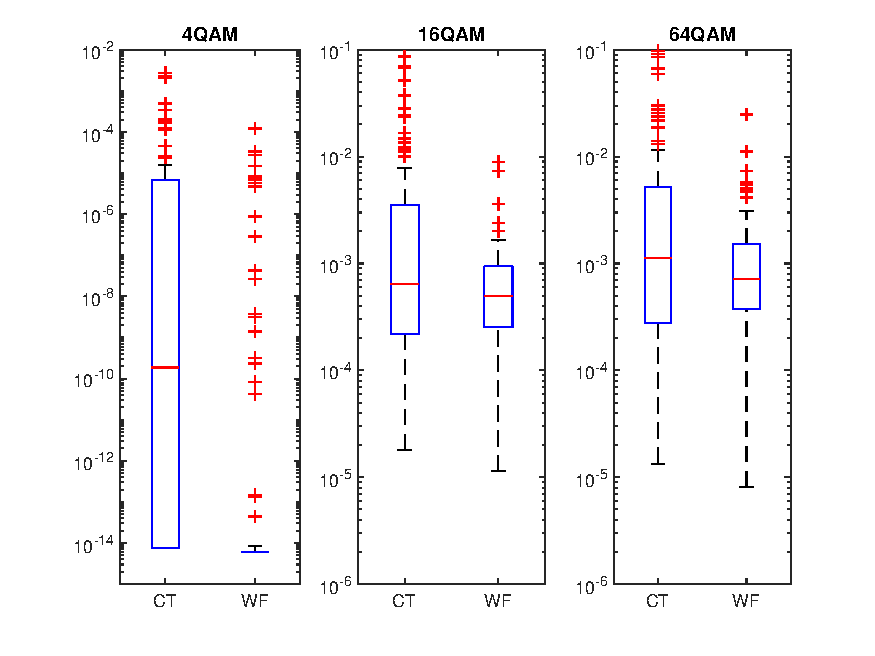
\includegraphics[width=0.8\linewidth]{./figs/WF_noiseless_mu1e3_M4L2_distr.pdf}
	\caption{Distribution of total interference after $T=1000$ iterations with different initialization approaches (Center Tap, and spectral initialization of WF), for different modulation schemes. }
	\label{fig:CMA_WF_ti_distribution}
\end{figure}


Now, we test the single-source recovery capabilities of WF, under different $L\times M$ system settings, different number of samples, and different QAM constellations, using the spectral initialization defined in Algorithm~\ref{alg:wf}. 

Figure~\ref{fig:CMA_WF_qpsk_L2M4} presents the cost function value and the total interference of each equalizer vs. outer iterations for each SNR value in a random experiment with QPSK transmissions, $L=2$ sources and $M=4$ receiving antennas. The left column shows the experiment using $K=200$ samples and the right column shows the experiment using $K=1000$ samples. This shows that the WF algorithm converges for all SNR values, even with a relatively small number of samples for gradient-descent schemes. The total interference decays rapidly over iterations, and the final interference obtained (when WF meets the stopping criterion) is less than 30dB reliably across all cases (the noiseless cases are mostly very low, but outliers can still be seen).

Figure~\ref{fig:CMA_WF_mods_L2M4} shows the behavior of WF for different modulation schemes, with $K=1000$, $L=2$ and $M=4$. The cost function seems to reach a minimum rather quickly for higher-order modulations, which is expected as these constellations have varying modulus, although the total interference steadily decreases to achieve less than 25dB over all scenarios.

Finally, Figure~\ref{fig:CMA_WF_size_qpsk} shows the effect of the system size $M\times L$ on the behavior of WF. A greater number of sources implies more interference to get rid of, effect that can be seen with a larger total interference across modulation schemes and SNR values. We also have to note that the stepsize had to be decreased for the larger system size, down to $\mu=2\cdot 10^{-4}$. This can be explained because the regions where the regularity condition holds are smaller, as the size of the basin of attraction $\epsilon$ (dependent on $B$) decreases with the amount of sources $L$, which in turn will make it harder for WF to land in the basin of attraction without theoretical guarantees of the initial iterate. Nevertheless, WF is capable of retrieving a source rather reliably under all conditions.

\begin{figure}
	\centering
	\begin{subfigure}[b]{0.45\textwidth}
		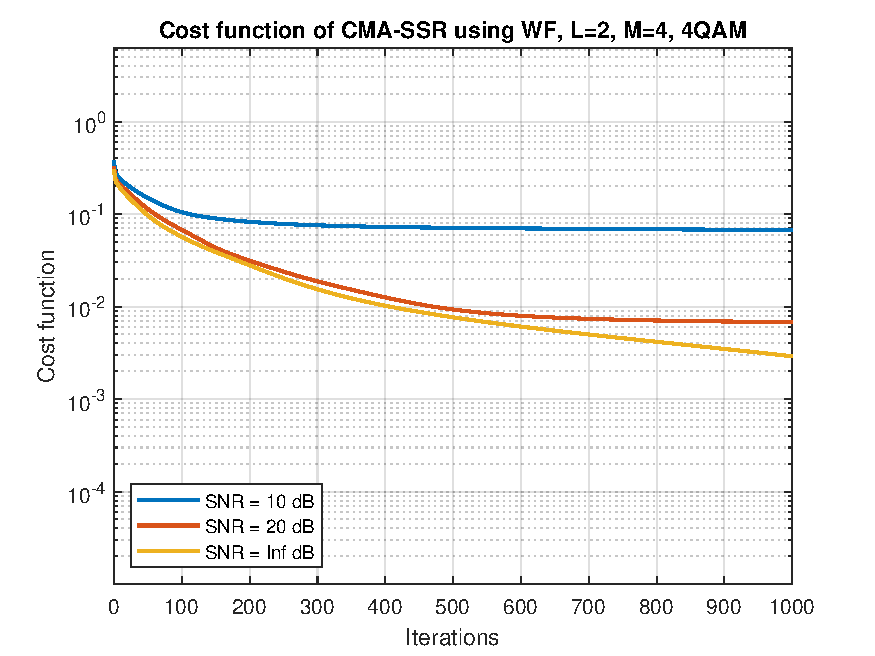
\includegraphics[width=\linewidth]{./figs/BF_WF_cost_4QAM_L=2_M=4_K=200.pdf}
		\subcaption{Cost function for $K=200$.}
		\label{fig:wf_cost200}
	\end{subfigure}
	\begin{subfigure}[b]{0.45\textwidth}
		% Caption before figure
		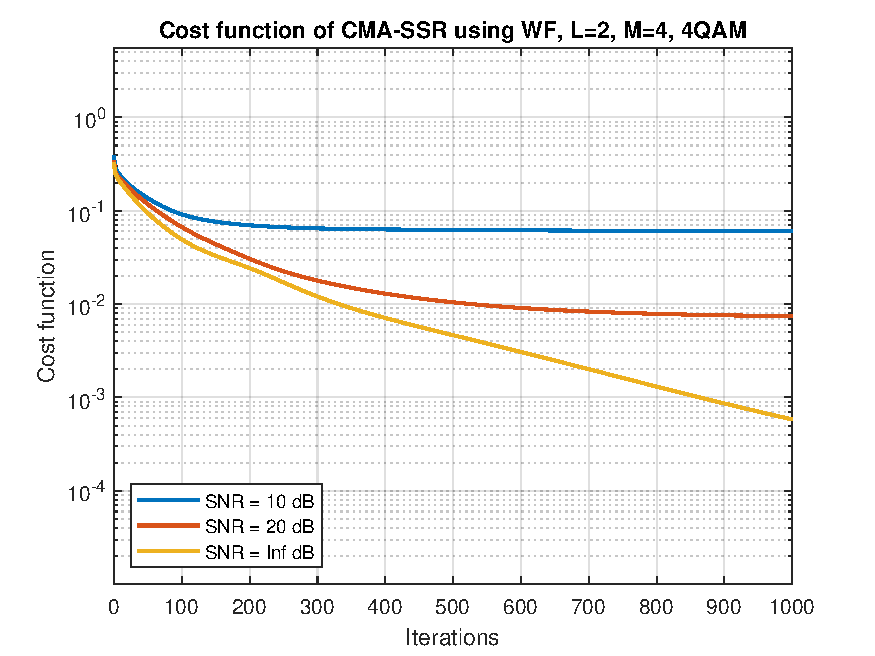
\includegraphics[width=\linewidth]{./figs/BF_WF_cost_4QAM_L=2_M=4_K=1000.pdf}
		\subcaption{Cost function for $K=1000$.}
		\label{fig:wf_cost1000}
	\end{subfigure}\\
	\begin{subfigure}[b]{0.45\textwidth}
		% Caption before figure
		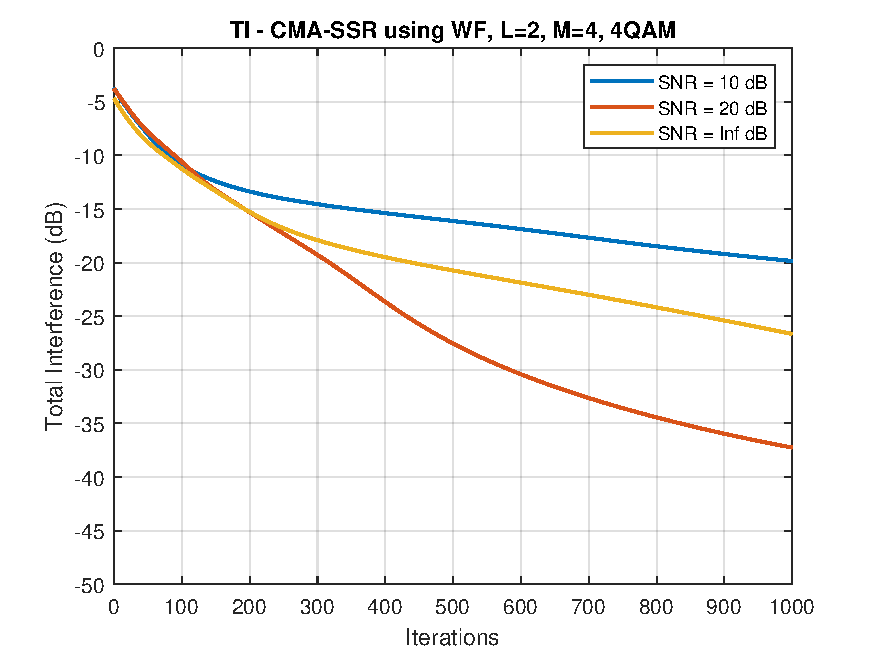
\includegraphics[width=\linewidth]{./figs/BF_WF_TI_4QAM_L=2_M=4_K=200.pdf}
		\subcaption{Total Interference for $K=200$.}
		\label{fig:wf_ti200}
	\end{subfigure}
	\begin{subfigure}[b]{0.45\textwidth}
		% Caption before figure
		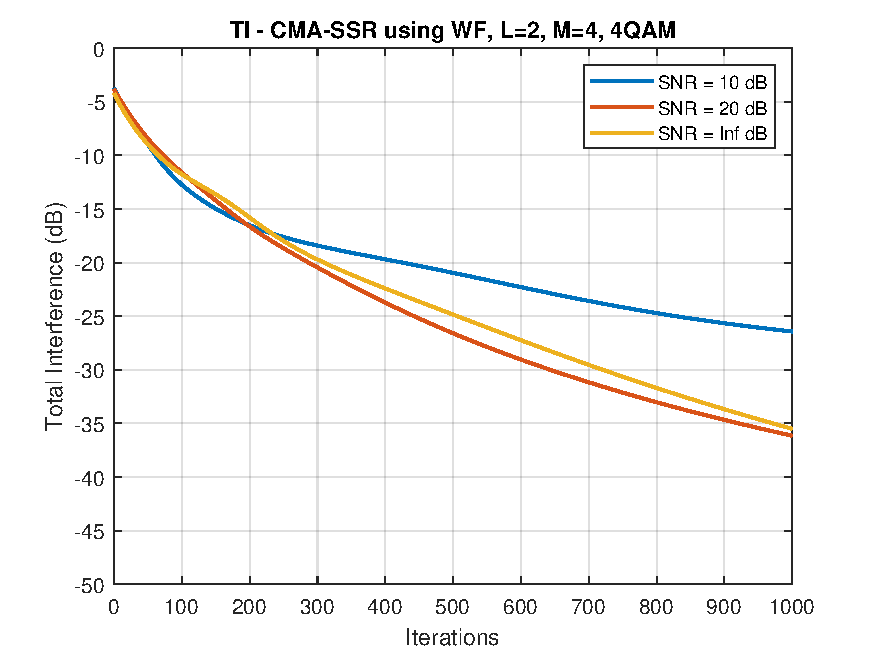
\includegraphics[width=\linewidth]{./figs/BF_WF_TI_4QAM_L=2_M=4_K=1000.pdf}
		\subcaption{Total Interference for $K=1000$.}
		\label{fig:wf_ti1000}
	\end{subfigure}
	\begin{subfigure}[b]{0.45\textwidth}
		% Caption before figure
		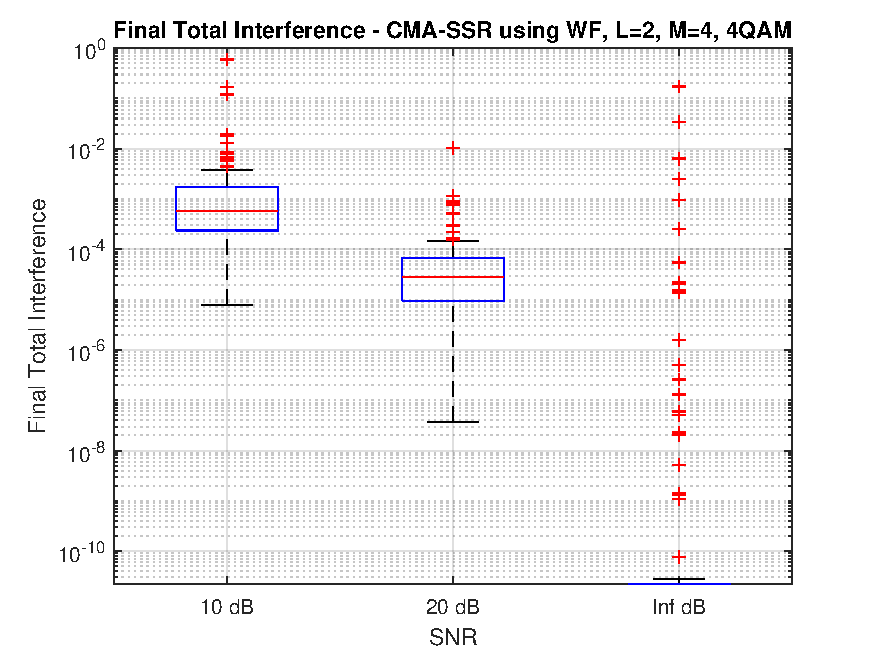
\includegraphics[width=\linewidth]{./figs/BF_WF_TIfinal_4QAM_L=2_M=4_K=200.pdf}
		\subcaption{Distribution of Interference for $K=200$.}
		\label{fig:wf_tidist200}
	\end{subfigure}
	\begin{subfigure}[b]{0.45\textwidth}
		% Caption before figure
		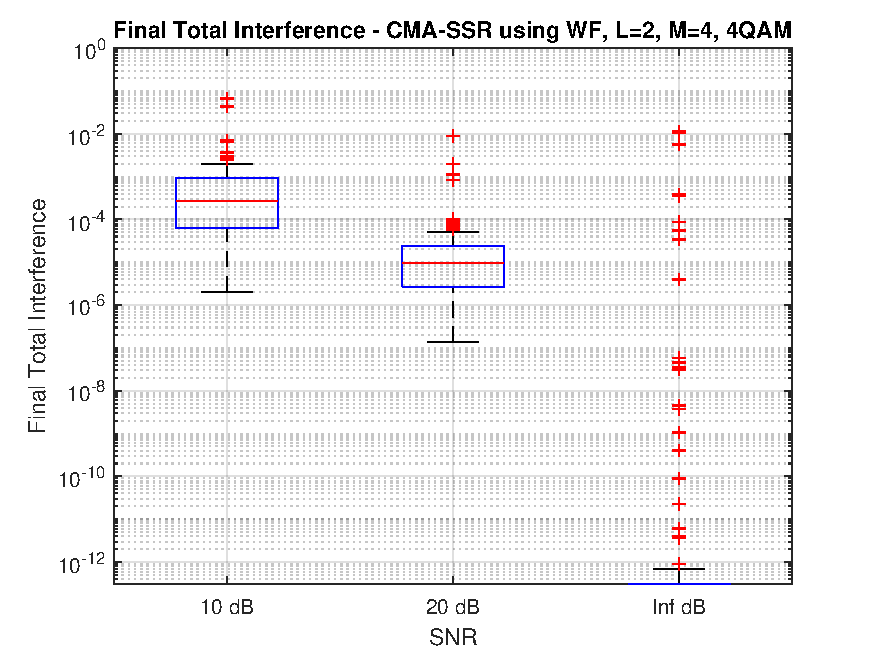
\includegraphics[width=\linewidth]{./figs/BF_WF_TIfinal_4QAM_L=2_M=4_K=1000.pdf}
		\subcaption{Distribution of interference for $K=1000$.}
		\label{fig:wf_tidist1000}
	\end{subfigure}
	\caption{Comparison between amount of samples for WF-SSR convergence. These are mean results from 100 independent runs of the algorithm, with QPSK modulation, $L=2$ and $M=4$.}
	\label{fig:CMA_WF_qpsk_L2M4}
\end{figure}

\begin{figure}
	\centering
	\begin{subfigure}[b]{0.45\textwidth}
		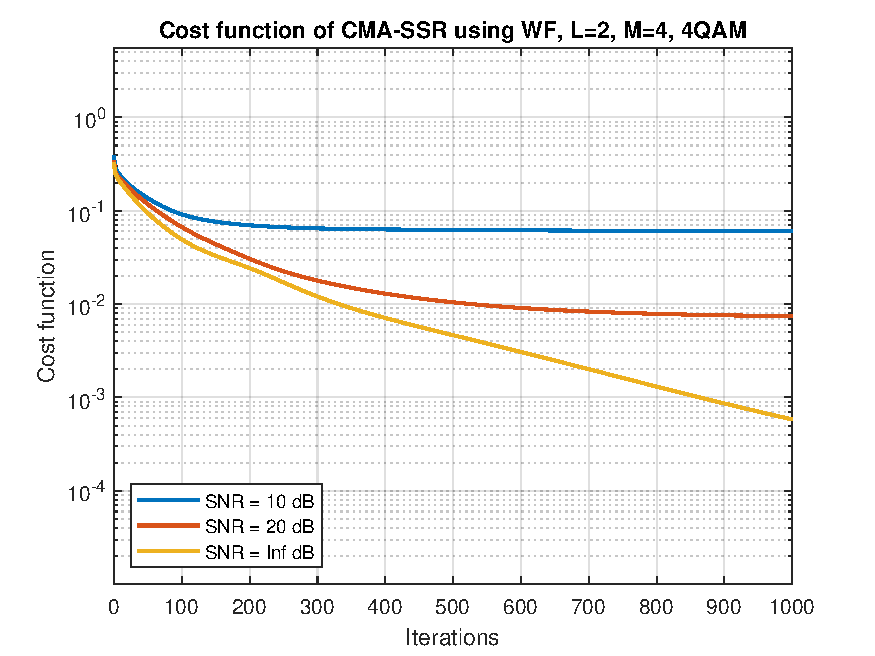
\includegraphics[width=\linewidth]{./figs/BF_WF_cost_4QAM_L=2_M=4_K=1000.pdf}
		\subcaption{Cost function for QPSK.}
		\label{fig:wf_costqpsk}
	\end{subfigure}
	\begin{subfigure}[b]{0.45\textwidth}
		% Caption before figure
		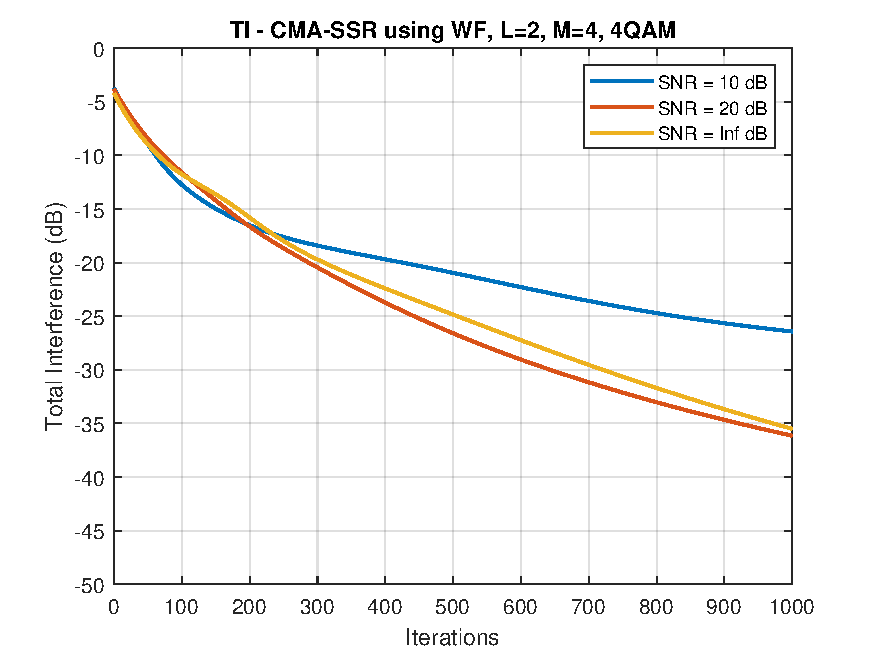
\includegraphics[width=\linewidth]{./figs/BF_WF_TI_4QAM_L=2_M=4_K=1000.pdf}
		\subcaption{Total interference for QPSK.}
		\label{fig:wf_ti_qpsk}
	\end{subfigure}\\
	\begin{subfigure}[b]{0.45\textwidth}
		% Caption before figure
		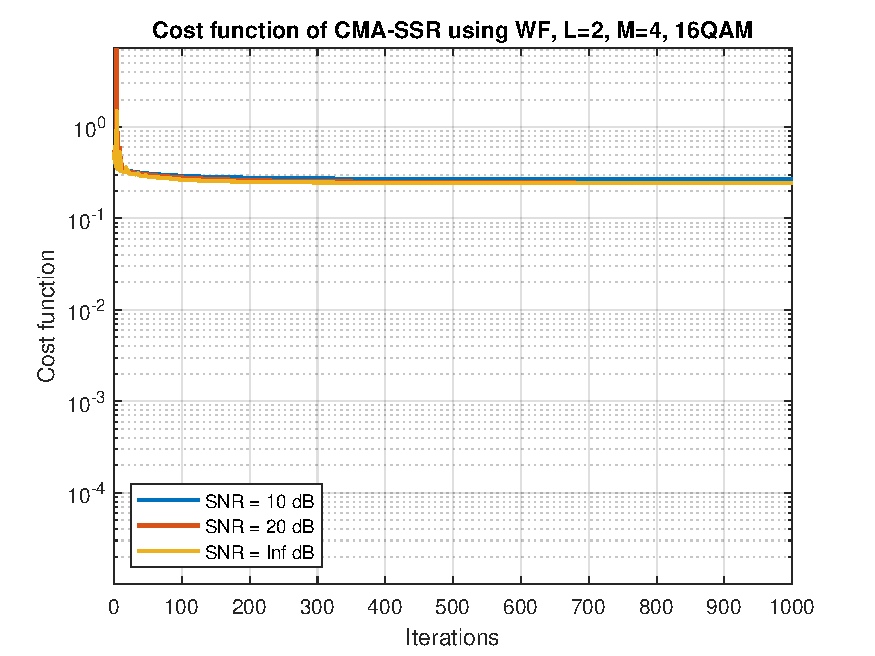
\includegraphics[width=\linewidth]{./figs/BF_WF_cost_16QAM_L=2_M=4_K=1000.pdf}
		\subcaption{Cost function for 16QAM.}
		\label{fig:wf_cost16}
	\end{subfigure}
	\begin{subfigure}[b]{0.45\textwidth}
		% Caption before figure
		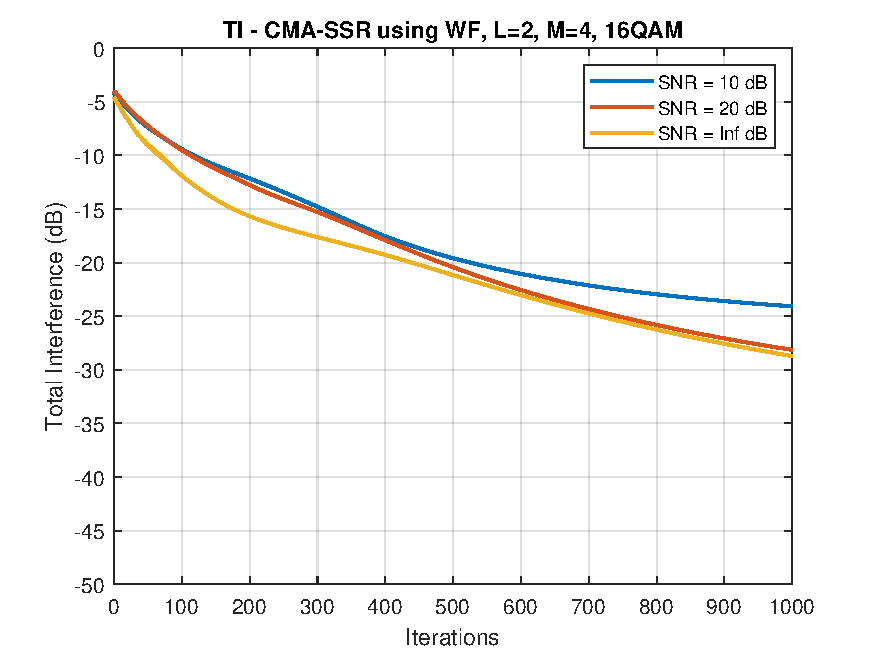
\includegraphics[width=\linewidth]{./figs/BF_WF_TI_16QAM_L=2_M=4_K=1000.pdf}
		\subcaption{Total interference for 16QAM.}
		\label{fig:wf_ti16}
	\end{subfigure}
	\begin{subfigure}[b]{0.45\textwidth}
		% Caption before figure
		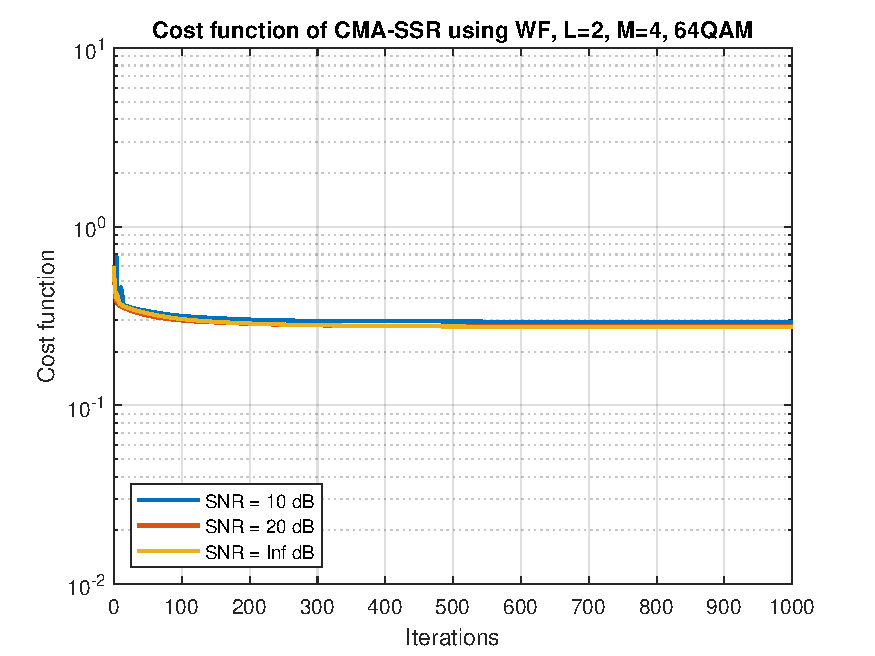
\includegraphics[width=\linewidth]{./figs/BF_WF_cost_64QAM_L=2_M=4_K=1000.pdf}
		\subcaption{Cost function for 64QAM.}
		\label{fig:wf_cost64}
	\end{subfigure}
	\begin{subfigure}[b]{0.45\textwidth}
		% Caption before figure
		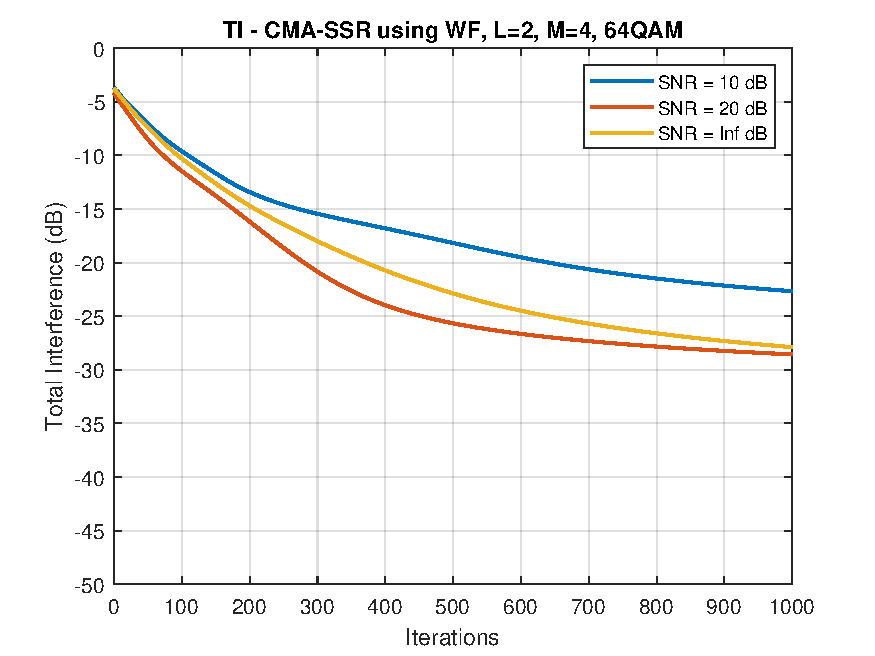
\includegraphics[width=\linewidth]{./figs/BF_WF_TI_64QAM_L=2_M=4_K=1000.pdf}
		\subcaption{Total interference for 64QAM.}
		\label{fig:wf_ti64}
	\end{subfigure}
	\caption{Comparison between modulations for WF-SSR convergence. These are mean results from 100 independent runs of the algorithm, with different SNR values, $K=1000$, $L=2$ and $M=4$.}
	\label{fig:CMA_WF_mods_L2M4}
\end{figure}

\begin{figure}
	\centering
	\begin{subfigure}[b]{0.45\textwidth}
		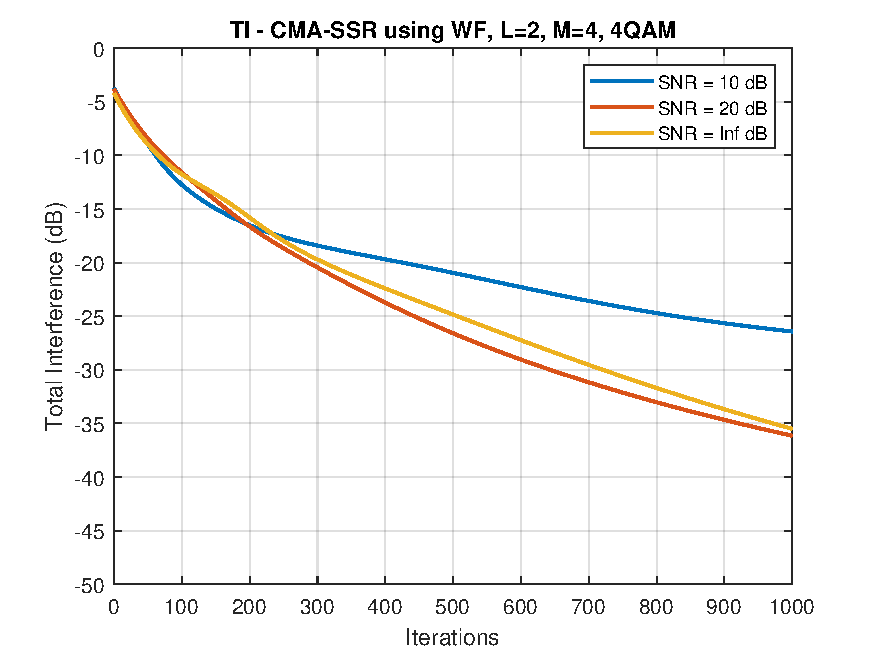
\includegraphics[width=\linewidth]{./figs/BF_WF_TI_4QAM_L=2_M=4_K=1000.pdf}
		\subcaption{TI, QPSK, $L=2$, $M=4$.}
		\label{fig:wf_ti4_24}
	\end{subfigure}
	\begin{subfigure}[b]{0.45\textwidth}
		% Caption before figure
		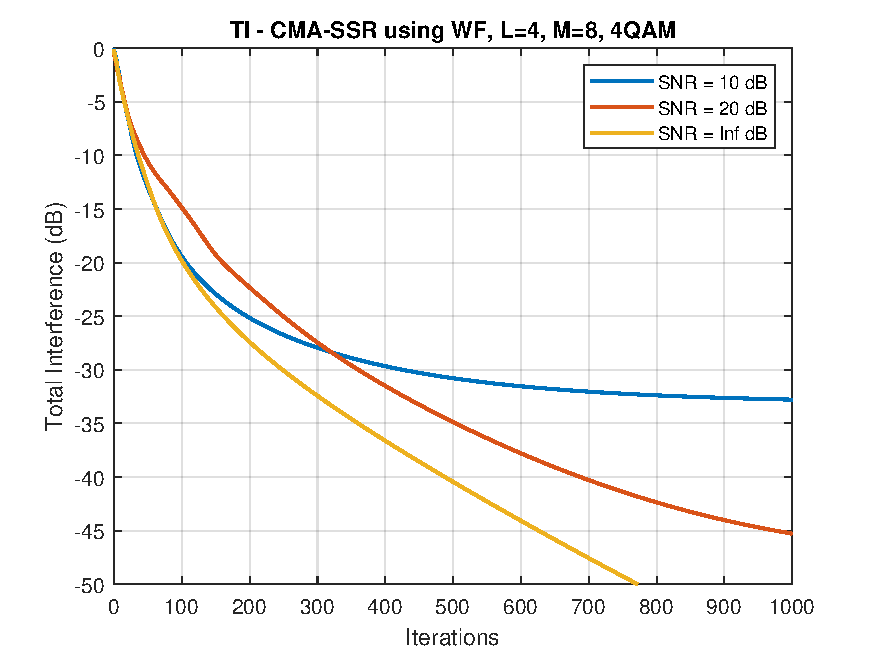
\includegraphics[width=\linewidth]{./figs/BF_WF_TI_4QAM_L=4_M=8_K=1000.pdf}
		\subcaption{TI, QPSK, $L=4$, $M=8$.}
		\label{fig:wf_ti4_48}
	\end{subfigure}\\
	\begin{subfigure}[b]{0.45\textwidth}
		% Caption before figure
		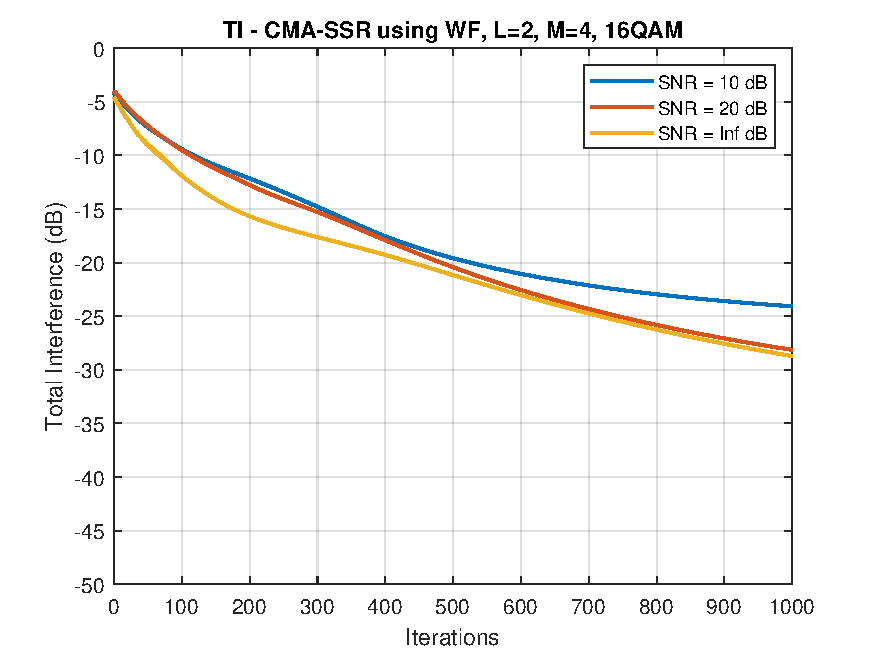
\includegraphics[width=\linewidth]{./figs/BF_WF_TI_16QAM_L=2_M=4_K=1000.pdf}
		\subcaption{TI, 16QAM, $L=2$, $M=4$.}
		\label{fig:wf_ti16_24}
	\end{subfigure}
	\begin{subfigure}[b]{0.45\textwidth}
		% Caption before figure
		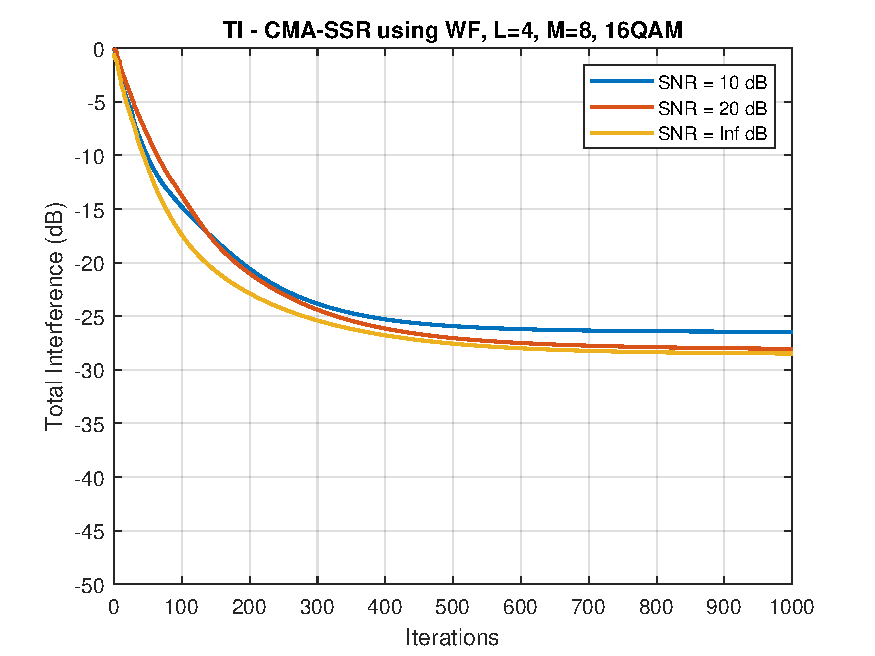
\includegraphics[width=\linewidth]{./figs/BF_WF_TI_16QAM_L=4_M=8_K=1000.pdf}
		\subcaption{TI, 16QAM, $L=42$, $M=8$.}
		\label{fig:wf_ti16_48}
	\end{subfigure}
	\begin{subfigure}[b]{0.45\textwidth}
		% Caption before figure
		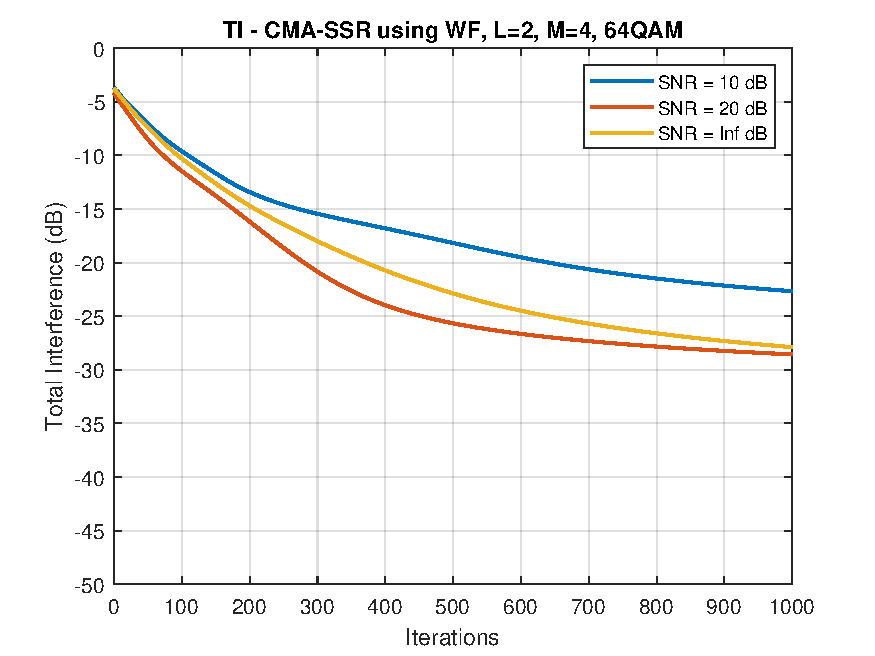
\includegraphics[width=\linewidth]{./figs/BF_WF_TI_64QAM_L=2_M=4_K=1000.pdf}
		\subcaption{TI, 64QAM, $L=2$, $M=4$.}
		\label{fig:wf_ti64_24}
	\end{subfigure}
	\begin{subfigure}[b]{0.45\textwidth}
		% Caption before figure
		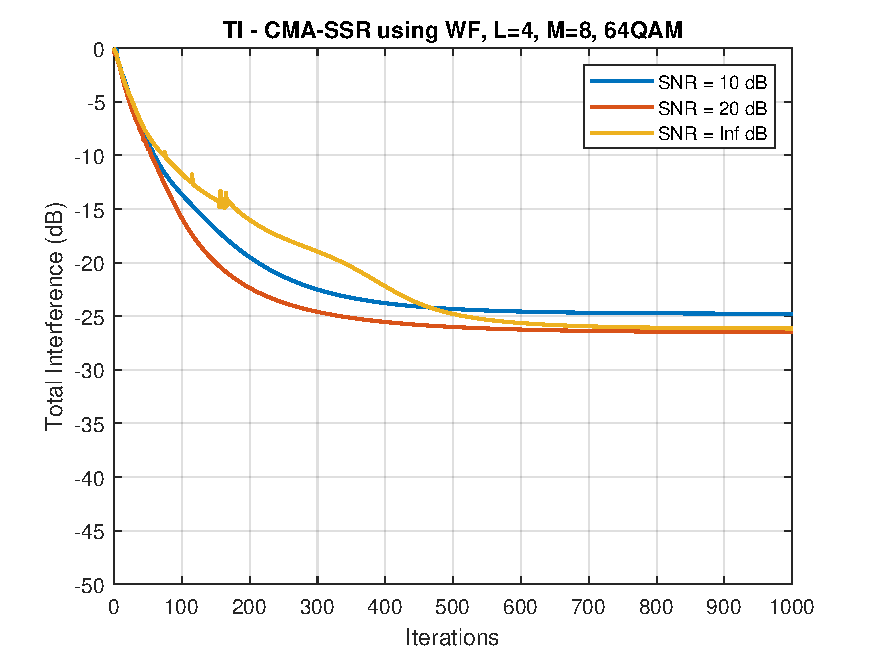
\includegraphics[width=\linewidth]{./figs/BF_WF_TI_64QAM_L=4_M=8_K=1000.pdf}
		\subcaption{TI, 64QAM, $L=4$, $M=8$.}
		\label{fig:wf_ti64_48}
	\end{subfigure}
	\caption{Comparison between system sizes for WF-SSR convergence. These are mean results from 100 independent runs of the algorithm, with different SNR values and $K=1000$.}
	\label{fig:CMA_WF_size_qpsk}
\end{figure}

\newpage
\subsection{Multiple source recovery}\label{sim:WF_MSR}
Here, we replicate some results from the single source recovery experiments, but recovering $J=2$ sources at a time. We furthermore set $\gamma_0=1$.

Figure~\ref{fig:CMA_WF_msr_qpsk_L2M4} presents the cost function value and the total interference of each equalizer vs. outer iterations for each SNR value in a random experiment with QPSK transmissions, $L=2$ sources and $M=4$ receiving antennas. The left column shows the experiment using $K=200$ samples and the right column shows the experiment using $K=1000$ samples. This shows that the WF-MSR algorithm converges for all SNR values, even with a relatively small number of samples for gradient-descent schemes. The total interference decays rapidly over iterations, and the final interference obtained (when WF meets the stopping criterion) is less than 25dB when $K=2--$ and less than 30dB for a larger number of samples.

Figure~\ref{fig:CMA_WF_msr_mods_L2M4} shows the behavior of WF for different modulation schemes, with $K=1000$, $L=2$ and $M=4$. The cost function seems to reach a stable value rather quickly for higher-order modulations, which is expected as these constellations have varying modulus, although again the total interference of both equalizers steadily decreases to achieve less than 25dB over all scenarios.

Finally, Figure~\ref{fig:CMA_WF_msr_size_qpsk} shows the effect of the system size $M\times L$ on the behavior of WF. A greater number of sources implies more interference to get rid of, effect that can be seen with a larger total interference across modulation schemes and SNR values. Again, we set a lower stepsize of $\mu=2\cdot 10^{-4}$ for the larger system size. Nevertheless, WF is capable of retrieving a source rather reliably under all conditions.

\begin{figure}
	\centering
	\begin{subfigure}[b]{0.45\textwidth}
		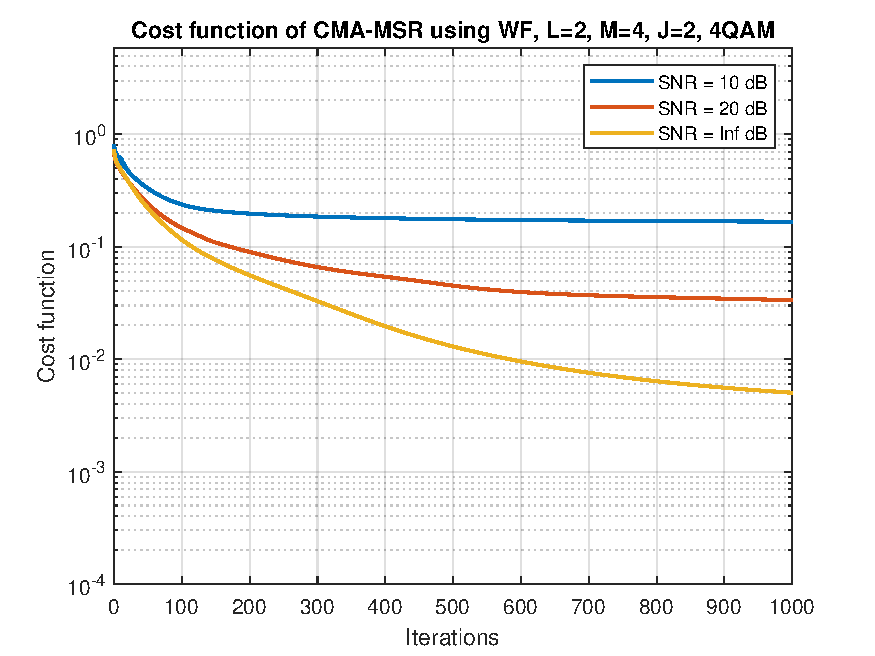
\includegraphics[width=\linewidth]{./figs/BF_WF_MSR_cost_4QAM_L=2_M=4_J=2_K=200.pdf}
		\subcaption{Cost function for $K=200$.}
		\label{fig:wf_msr_cost200}
	\end{subfigure}
	\begin{subfigure}[b]{0.45\textwidth}
		% Caption before figure
		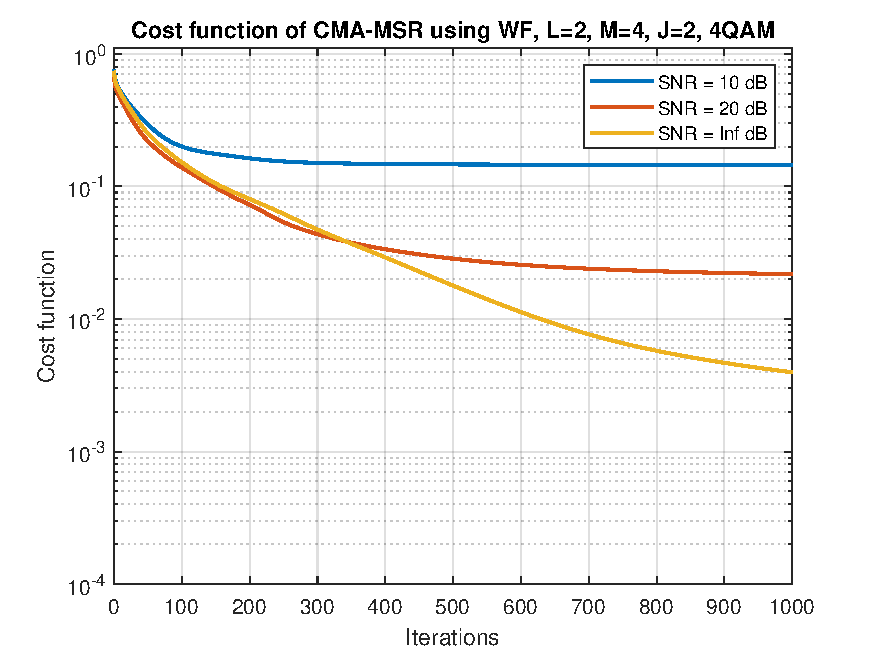
\includegraphics[width=\linewidth]{./figs/BF_WF_MSR_cost_4QAM_L=2_M=4_J=2_K=1000.pdf}
		\subcaption{Cost function for $K=1000$.}
		\label{fig:wf_msr_cost1000}
	\end{subfigure}\\
	\begin{subfigure}[b]{0.45\textwidth}
		% Caption before figure
		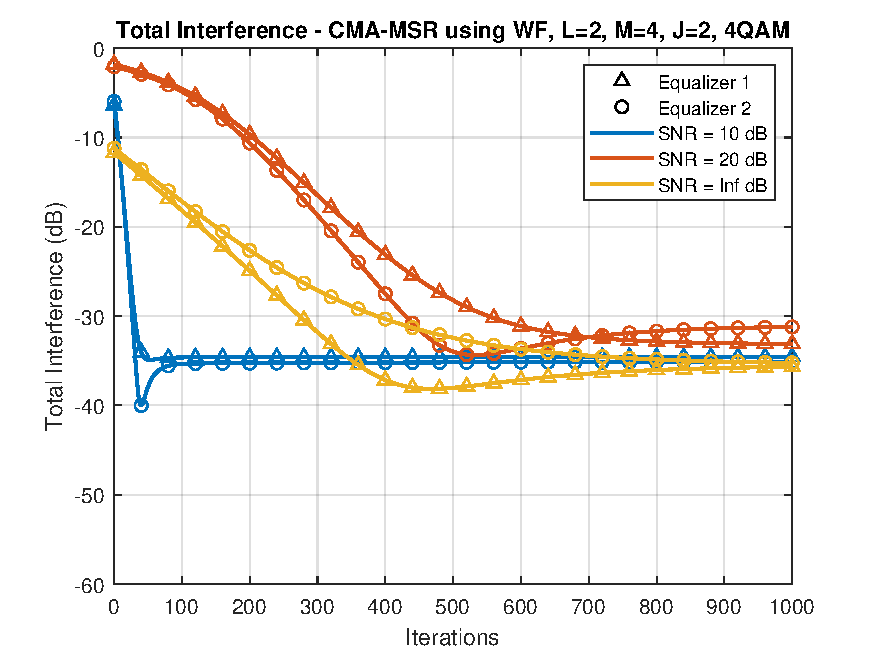
\includegraphics[width=\linewidth]{./figs/BF_WF_MSR_TI_4QAM_L=2_M=4_J=2_K=200.pdf}
		\subcaption{Total Interference for $K=200$.}
		\label{fig:wf_msr_ti200}
	\end{subfigure}
	\begin{subfigure}[b]{0.45\textwidth}
		% Caption before figure
		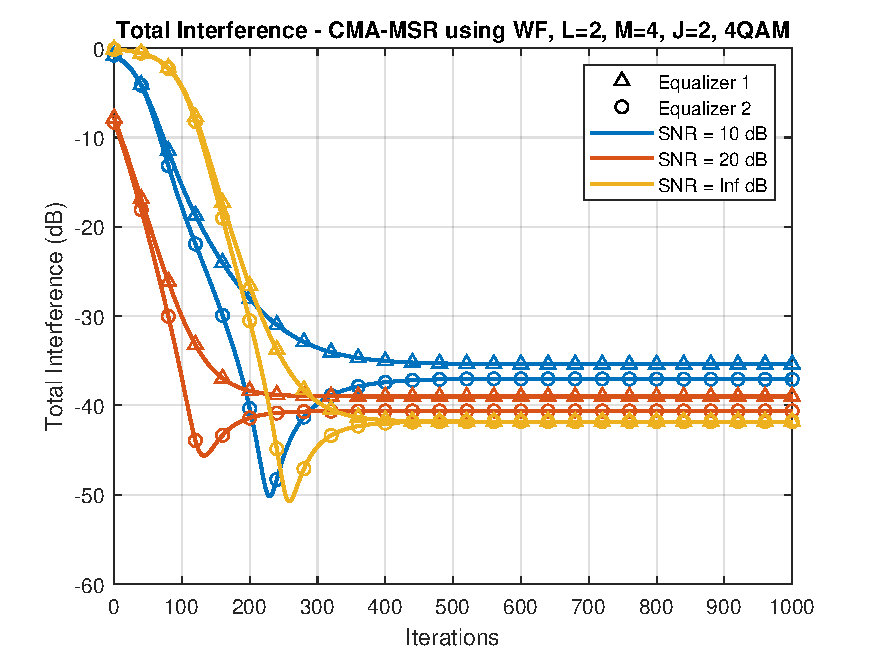
\includegraphics[width=\linewidth]{./figs/BF_WF_MSR_TI_4QAM_L=2_M=4_J=2_K=1000.pdf}
		\subcaption{Total Interference for $K=1000$.}
		\label{fig:wf_msr_ti1000}
	\end{subfigure}
	\begin{subfigure}[b]{0.45\textwidth}
		% Caption before figure
		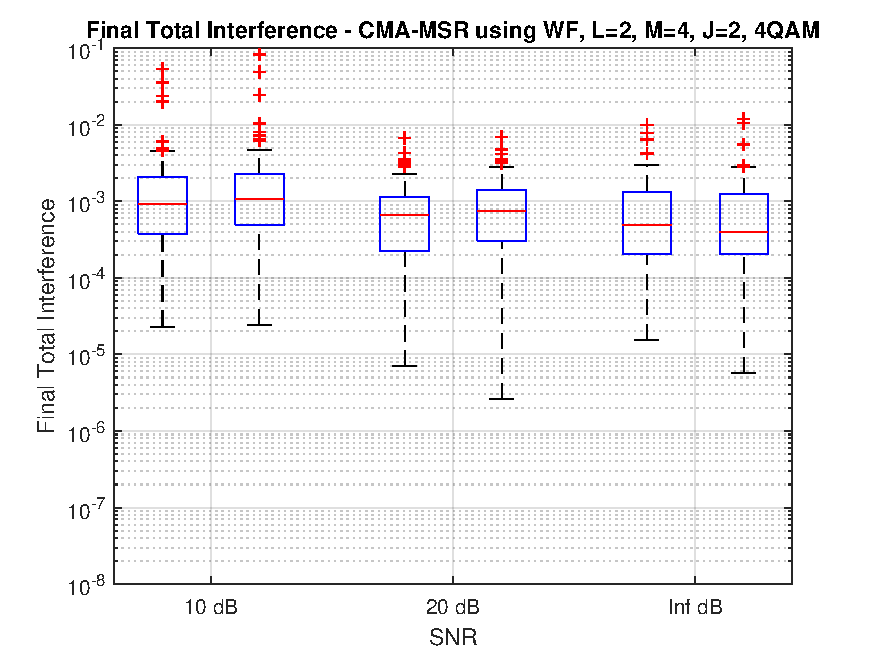
\includegraphics[width=\linewidth]{./figs/BF_WF_MSR_TIfinal_4QAM_L=2_M=4_J=2_K=200.pdf}
		\subcaption{Distribution of Interference for $K=200$.}
		\label{fig:wf_msr_tidist200}
	\end{subfigure}
	\begin{subfigure}[b]{0.45\textwidth}
		% Caption before figure
		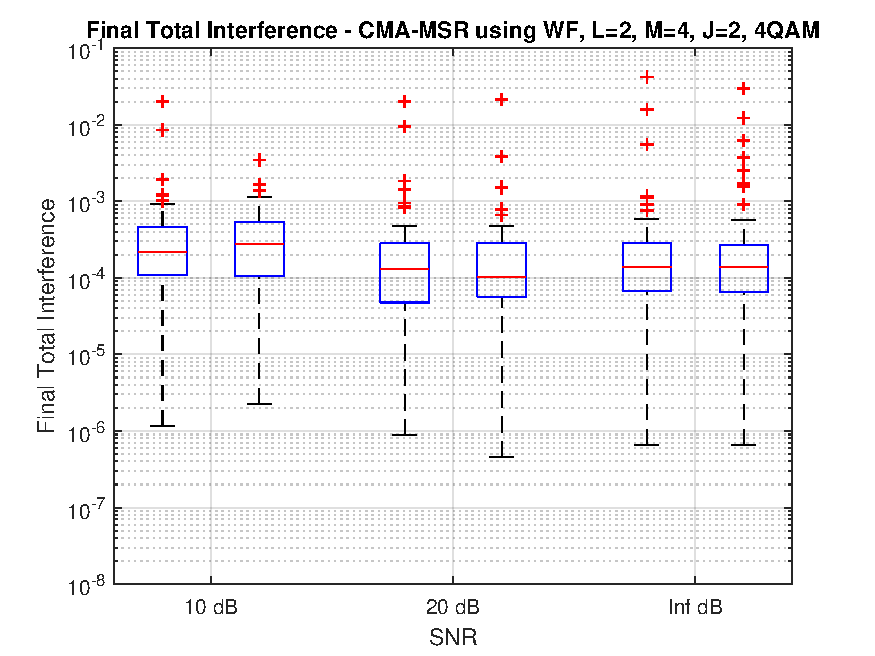
\includegraphics[width=\linewidth]{./figs/BF_WF_MSR_TIfinal_4QAM_L=2_M=4_J=2_K=1000.pdf}
		\subcaption{Distribution of interference for $K=1000$.}
		\label{fig:wf_msr_tidist1000}
	\end{subfigure}
	\caption{Comparison between amount of samples for WF-MSR convergence. These are mean results from 100 independent runs of the algorithm, with QPSK modulation, $L=2$, $J=2$ and $M=4$.}
	\label{fig:CMA_WF_msr_qpsk_L2M4}
\end{figure}

\begin{figure}
	\centering
	\begin{subfigure}[b]{0.45\textwidth}
		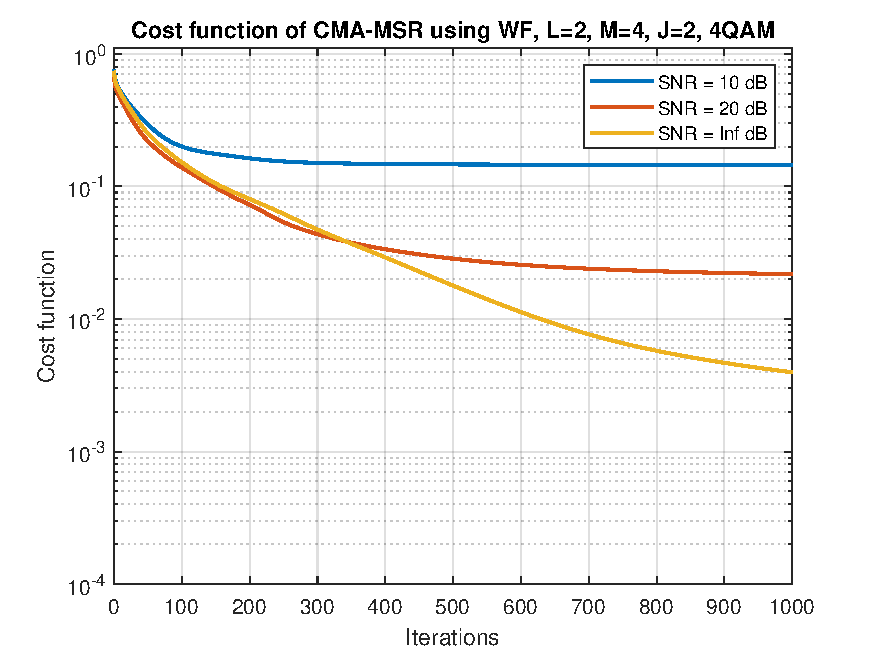
\includegraphics[width=\linewidth]{./figs/BF_WF_MSR_cost_4QAM_L=2_M=4_J=2_K=1000.pdf}
		\subcaption{Cost function for QPSK.}
		\label{fig:wf_msr_costqpsk}
	\end{subfigure}
	\begin{subfigure}[b]{0.45\textwidth}
		% Caption before figure
		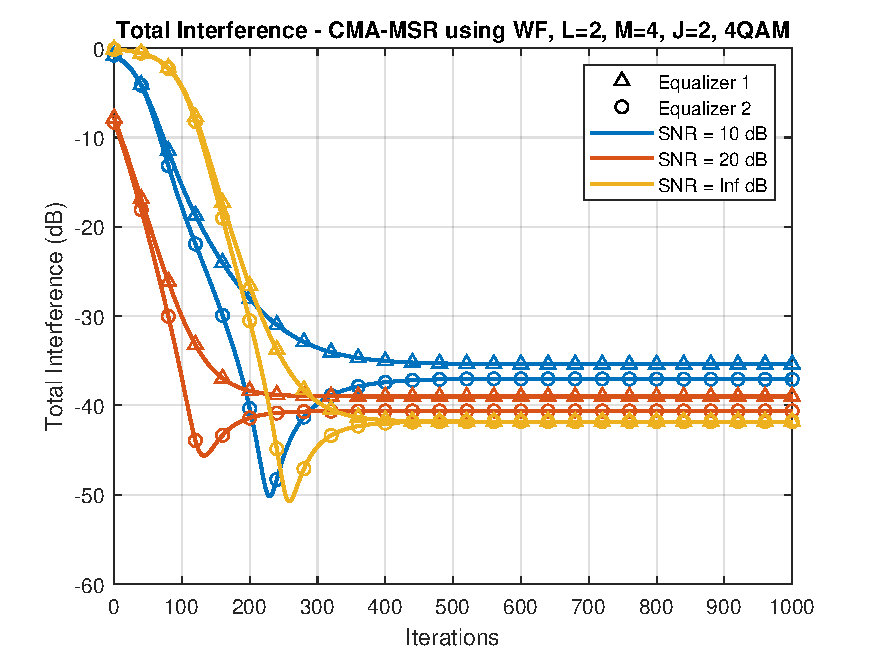
\includegraphics[width=\linewidth]{./figs/BF_WF_MSR_TI_4QAM_L=2_M=4_J=2_K=1000.pdf}
		\subcaption{Total interference for QPSK.}
		\label{fig:wf_msr_ti_qpsk}
	\end{subfigure}\\
	\begin{subfigure}[b]{0.45\textwidth}
		% Caption before figure
		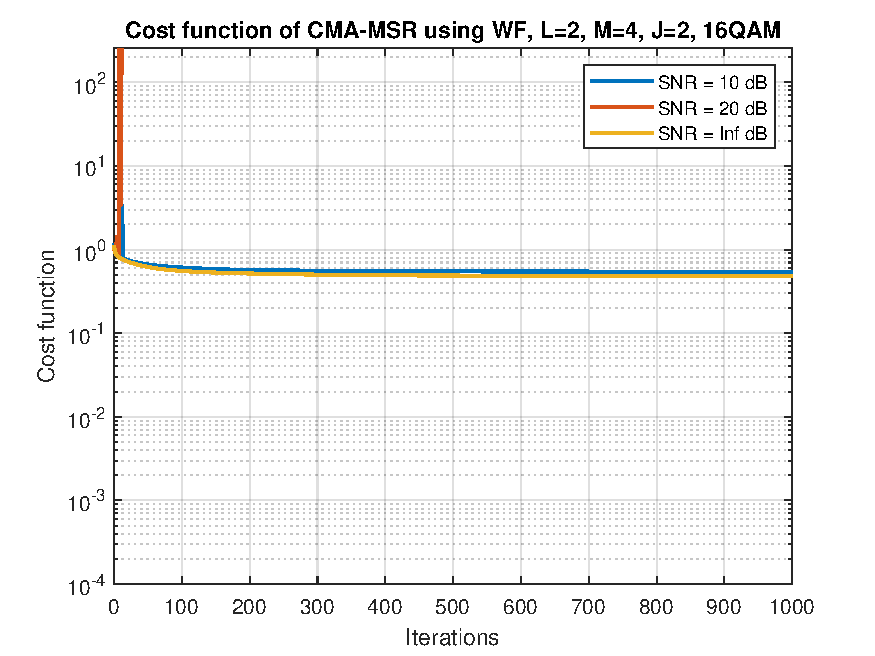
\includegraphics[width=\linewidth]{./figs/BF_WF_MSR_cost_16QAM_L=2_M=4_J=2_K=1000.pdf}
		\subcaption{Cost function for 16QAM.}
		\label{fig:wf_msr_cost16}
	\end{subfigure}
	\begin{subfigure}[b]{0.45\textwidth}
		% Caption before figure
		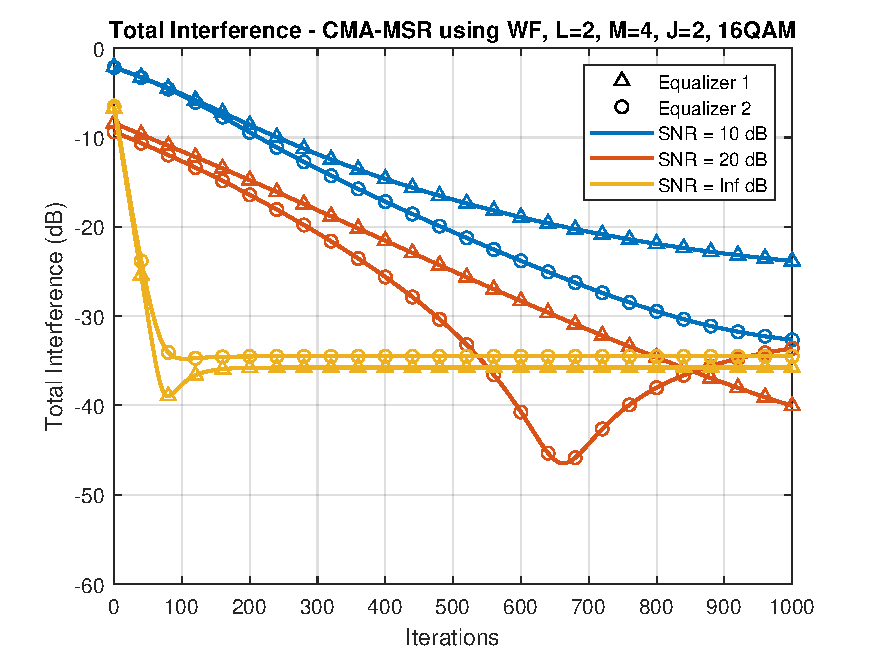
\includegraphics[width=\linewidth]{./figs/BF_WF_MSR_TI_16QAM_L=2_M=4_J=2_K=1000.pdf}
		\subcaption{Total interference for 16QAM.}
		\label{fig:wf_msr_ti16}
	\end{subfigure}
	\begin{subfigure}[b]{0.45\textwidth}
		% Caption before figure
		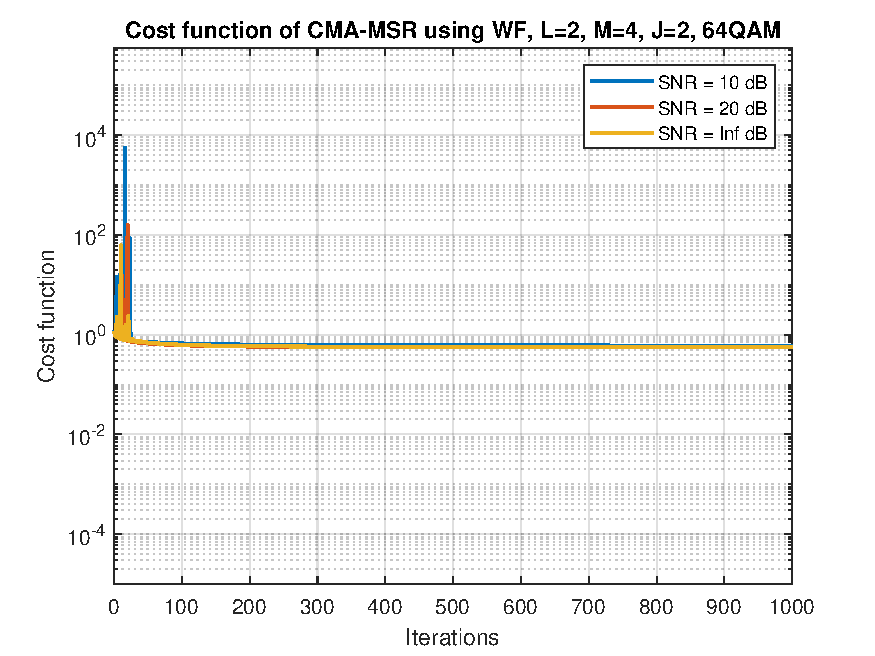
\includegraphics[width=\linewidth]{./figs/BF_WF_MSR_cost_64QAM_L=2_M=4_J=2_K=1000.pdf}
		\subcaption{Cost function for 64QAM.}
		\label{fig:wf_msr_cost64}
	\end{subfigure}
	\begin{subfigure}[b]{0.45\textwidth}
		% Caption before figure
		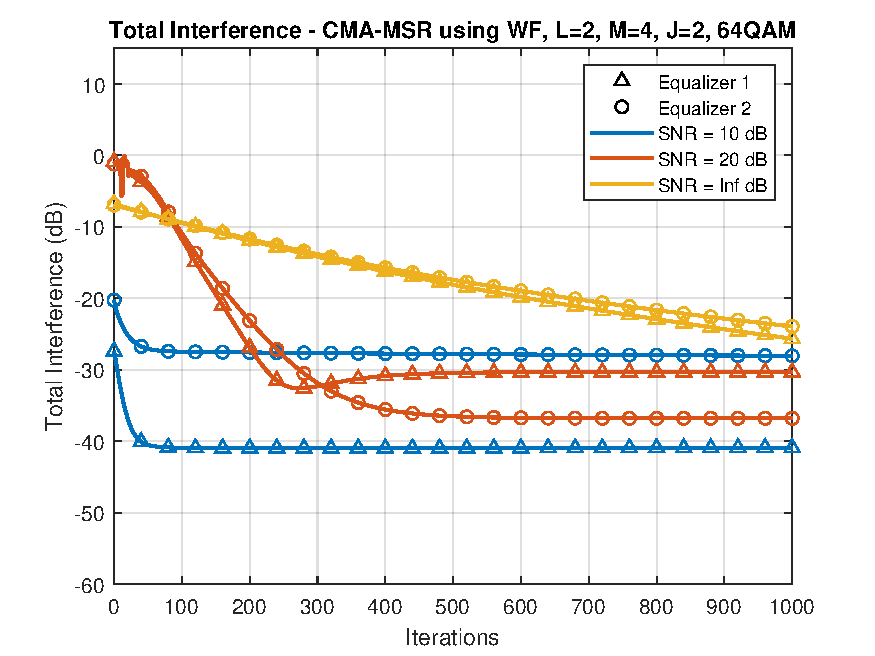
\includegraphics[width=\linewidth]{./figs/BF_WF_MSR_TI_64QAM_L=2_M=4_J=2_K=1000.pdf}
		\subcaption{Total interference for 64QAM.}
		\label{fig:wf_msr_ti64}
	\end{subfigure}
	\caption{Comparison between modulations for WF-MSR convergence. These are mean results from 100 independent runs of the algorithm, with different SNR values, $K=1000$, $L=2$, $J=2$ and $M=4$.}
	\label{fig:CMA_WF_msr_mods_L2M4}
\end{figure}

\begin{figure}
	\centering
	\begin{subfigure}[b]{0.45\textwidth}
		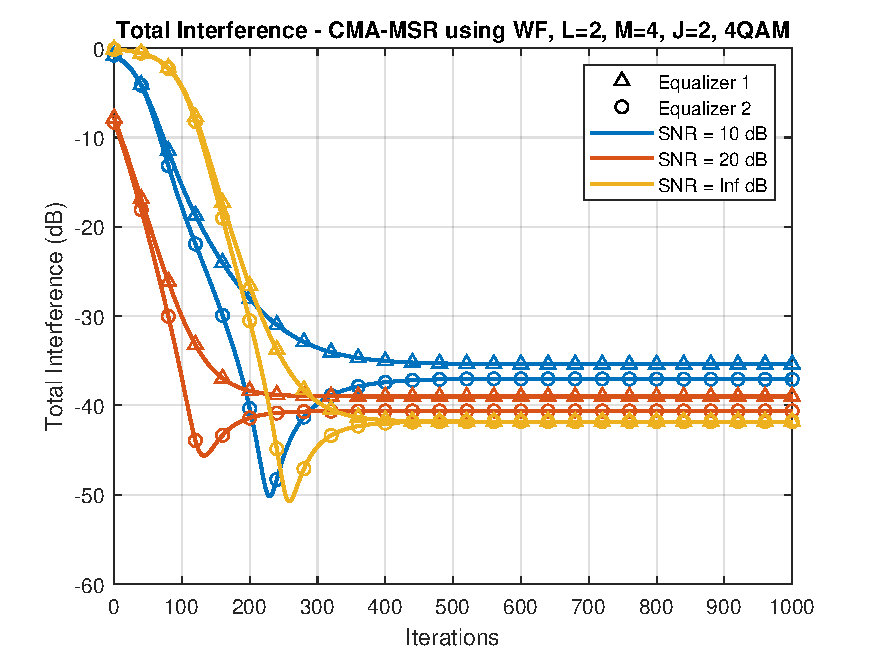
\includegraphics[width=\linewidth]{./figs/BF_WF_MSR_TI_4QAM_L=2_M=4_J=2_K=1000.pdf}
		\subcaption{TI, QPSK, $L=2$, $M=4$.}
		\label{fig:wf_msr_ti4_24}
	\end{subfigure}
	\begin{subfigure}[b]{0.45\textwidth}
		% Caption before figure
		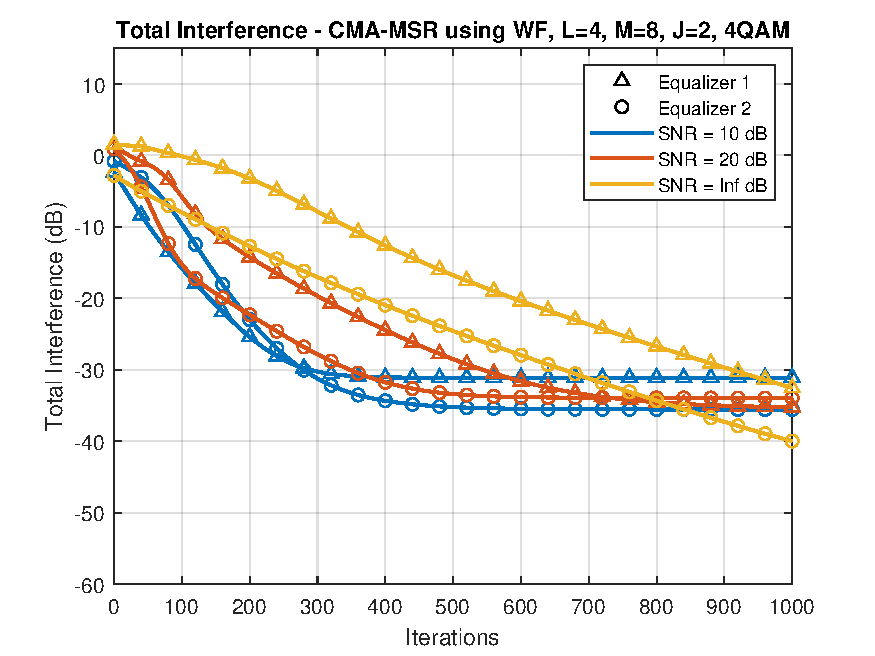
\includegraphics[width=\linewidth]{./figs/BF_WF_MSR_TI_4QAM_L=4_M=8_J=2_K=1000.pdf}
		\subcaption{TI, QPSK, $L=4$, $M=8$.}
		\label{fig:wf_msr_ti4_48}
	\end{subfigure}\\
	\begin{subfigure}[b]{0.45\textwidth}
		% Caption before figure
		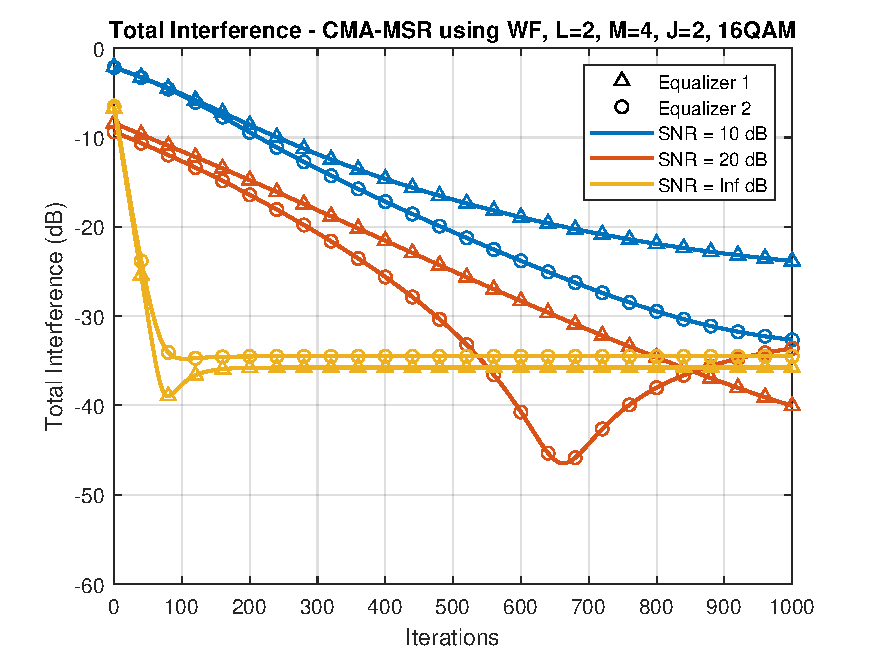
\includegraphics[width=\linewidth]{./figs/BF_WF_MSR_TI_16QAM_L=2_M=4_J=2_K=1000.pdf}
		\subcaption{TI, 16QAM, $L=2$, $M=4$.}
		\label{fig:wf_msr_ti16_24}
	\end{subfigure}
	\begin{subfigure}[b]{0.45\textwidth}
		% Caption before figure
		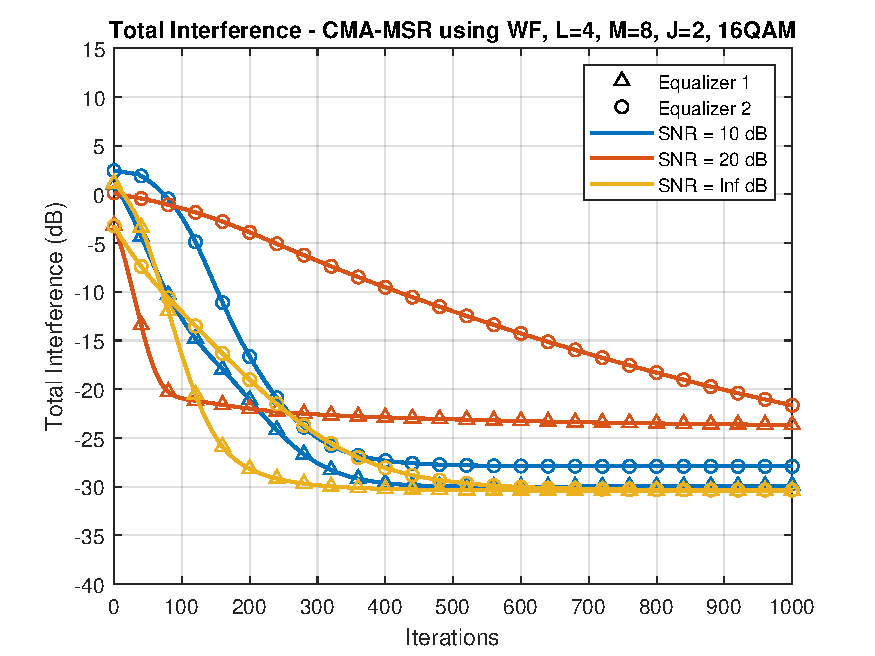
\includegraphics[width=\linewidth]{./figs/BF_WF_MSR_TI_16QAM_L=4_M=8_J=2_K=1000.pdf}
		\subcaption{TI, 16QAM, $L=42$, $M=8$.}
		\label{fig:wf_msr_ti16_48}
	\end{subfigure}
	\begin{subfigure}[b]{0.45\textwidth}
		% Caption before figure
		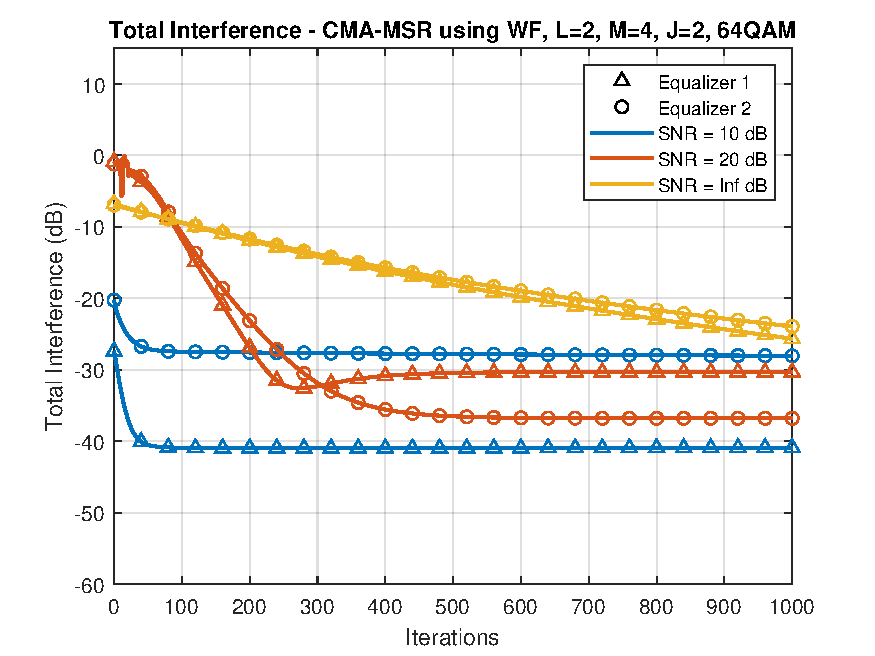
\includegraphics[width=\linewidth]{./figs/BF_WF_MSR_TI_64QAM_L=2_M=4_J=2_K=1000.pdf}
		\subcaption{TI, 64QAM, $L=2$, $M=4$.}
		\label{fig:wf_msr_ti64_24}
	\end{subfigure}
	\begin{subfigure}[b]{0.45\textwidth}
		% Caption before figure
		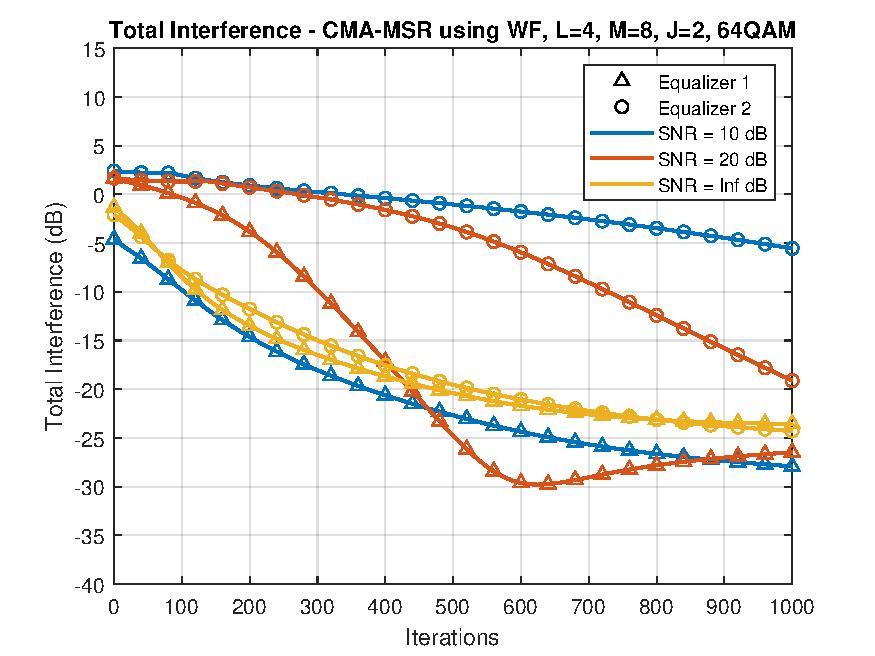
\includegraphics[width=\linewidth]{./figs/BF_WF_MSR_TI_64QAM_L=4_M=8_J=2_K=1000.pdf}
		\subcaption{TI, 64QAM, $L=4$, $M=8$.}
		\label{fig:wf_msr_ti64_48}
	\end{subfigure}
	\caption{Comparison between system sizes for WF-MSR convergence. These are mean results from 100 independent runs of the algorithm, with different SNR values, $J=2$ and $K=1000$.}
	\label{fig:CMA_WF_msr_size_qpsk}
\end{figure}